\section{REAL CASE STUDY: OPTIMAL HEATING SYSTEM SCHEDULING} In this section we show an application of DPC to a real case study. In particular, in the following we first describe the plant structure, then we provide both data-based and EnergyPlus model of such a plant to be used for control and performance comparison, and finally we show results of the closed-loop simulations.

\subsection{Description of the house}\label{SS:descriptionHouse}
The chosen case study is a detached off-grid two-story residential house, located in the outskirt of L'Aquila (coordinates $42\degree$ $16'$ latitude and $13\degree$ $32'$ longitude), Italy and is shown in Figure \ref{F:house}. The building, inhabited by the two owners, has a main north-south orientation and it is composed by a heated ground floor, that includes $4$ rooms, and an attic without heating system. Therefore, although the gross area of the house is equal to $209.5\,m^2$, the heated gross area is equal to $112.4\,m^2$. 


\begin{figure}[h!]
	\begin{center}
		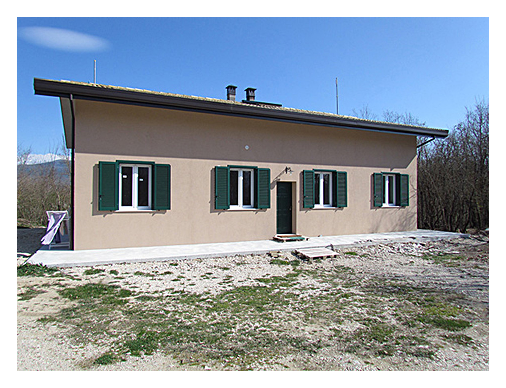
\includegraphics[width=24pc]{figures/Vista_sud.eps}
		\caption{Off-grid residential house.}
		\captionsetup{justification=centering}
		\label{F:house}
	\end{center}
\end{figure}

Thanks to the off-grid characteristic, the technological plants guarantee the complete energy self-sufficiency of the building. Indeed the house, equipped with a biomass boiler, a solar thermal plant, a stand-alone photovoltaic system, black water and rainwater reuse systems and as well for water supply, has a complete independence from the utilities.   
The bearing structure of the house is made of reinforced concrete and EPS (expanded polystyrene) insulation, while the building envelope is composed by prefabricated wood-cement blocks, shown in Figure \ref{F:houseSection}, with EPS and graphite insulation, that allow low thermal fluxes thanks to their high thermal performance. The thermal performance of a wood-cement block, with similar geometry, was investigated in a previous work \cite{Nardi2016}, both with experimental and numerical approach.

\begin{figure}[h!]
	\begin{center}
		\subfigure[Walls.]{
			\label{F:houseSection1}
			\centering
			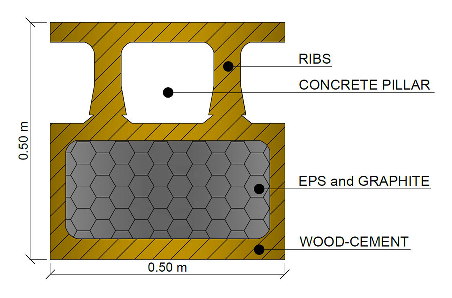
\includegraphics[width=24pc]{figures/blocco_parete_rev01.eps}
		}
		\subfigure[Floor and roof.]{
			\label{F:houseSection2}
			\centering
			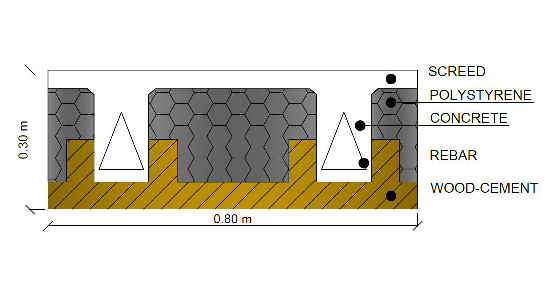
\includegraphics[width=24pc]{figures/blocco_solaio_rev01.eps}
		}
	\end{center}
	\caption{Cross-sections of the wood-cement blocks.}
	\captionsetup{justification=centering}
	\label{F:houseSection}
\end{figure}
The heating system of the building, that supplies the thermal energy required in winter season, is a hydronic system consisting of a vegetable biomass boiler, with a manual ON/OFF, a constant-flow pump station, and tubular steel radiators as shown in Figure \ref{F:housePlantScheme}. The standard biomass boiler has an efficiency of $83.5\%$ with $16.5\ kW$ of thermal power transferred to the water, without gas-flame modulation. The heat transfer fluid distribution is realized through a manifold circuit, that supplies the radiators placed in the various rooms of the house. The energy needs for the domestic hot water (DHW) are covered by the same boiler, coupled with a solar thermal plant. It is worth noting that, in this work, the thermal energy needed for the domestic hot water production is neglected. 

\begin{figure}[h!]
	\begin{center}
		\includegraphics[width=26pc]{figures/Schema_di_impianto.eps}
		\caption{Technological plant scheme of the use case.}
		\captionsetup{justification=centering}
		\label{F:housePlantScheme}
	\end{center}
\end{figure}
For a thorough knowledge of the building thermal behavior, an in-situ analysis was carried out. Temperature measuring devices, completely self-produced at the “G. Parolini Lab” of the University of L'Aquila \cite{Pantoli2017}, mainly based on an $ATmega 2560$ microcontroller and $DS18B20$ temperature probes (temperature range from $-55.0\degree C$ to $125.0\degree C$ with an accuracy of $\pm 0.5\degree C$), were employed to acquire the ambient temperatures of the four differently oriented rooms of the house as shown in Figure \ref{F:houseFloors}. The probes positions were chosen to optimize the data acquisition and to minimize the discomfort of the occupants in the house. Furthermore, as can be seen in Figures \ref{F:housePlantScheme} and \ref{F:houseFloors} (COMMENT: NOT CLEAR WHERE THE SENSORS ARE IN THE FIGURES. MORE DETAILS NEEDED), a commercial heat meter (temperature range from $10.0\degree C$ to $90.0\degree C$ with an accuracy of $\pm 0.05\degree C$) was installed downstream of the biomass boiler to measure the produced thermal energy. All the measuring devices have been set with a data acquisition rate equal to $10$ minutes, from March $11^{th}$ $2016$ to May $15^{th}$ $2016$.
\begin{figure}[h!]
	\begin{center}
		\subfigure[Ground floor.]{
			\label{F:houseGroundFloor}
			\centering
			\includegraphics[width=26pc]{figures/Arch_PT_e_sonde.eps}
		}
		\subfigure[Attic.]{
			\label{F:houseAttic}
			\centering
			\hspace{-1.6cm}
			\includegraphics[width=22.8pc]{figures/Arch_P1.eps}
		}
	\end{center}
	\caption{Layout of the house and probes placement. Legend: red circle for ambient temperature; orange circle for heat meter.}
	\captionsetup{justification=centering}
	\label{F:houseFloors}
\end{figure}

The collected data are used in the following to create both an EnergyPlus and a random forest model for the energy consumption of the house. These models will be used for performance comparison of DPC with respect to a classical bang-bang controller. In particular DPC will be set up to provide an optimal ON/OFF scheduling policy for the heating system in order to save energy while guaranteeing thermal comfort for the occupants. To this aim, we also create random forest models for power consumption and room temperatures to be used in the closed-loop simulations. 

\subsection{EnergyPlus model}\label{SS:energyPlusmodel}
To assess the energy performance of the use case's heating system, the EnergyPlus engine coupled with DesignBuilder modeling environment was employed. Based on the weather data provided by CETEMPS – Centre of Excellence \cite{CETEMPS}, shown in Figure \ref{F:houseExternalWeather}, the performed dynamic simulation was based on a weather file specifically created for L'Aquila, that according to the K\"{o}ppen-Geiger climate classification, has a warm temperate climate (Csa, Cfa and Csb) \cite{Peel2007}. (COMMENT: TO BE BETTER WRITTEN)

\begin{figure}[h!]
	\begin{center}
		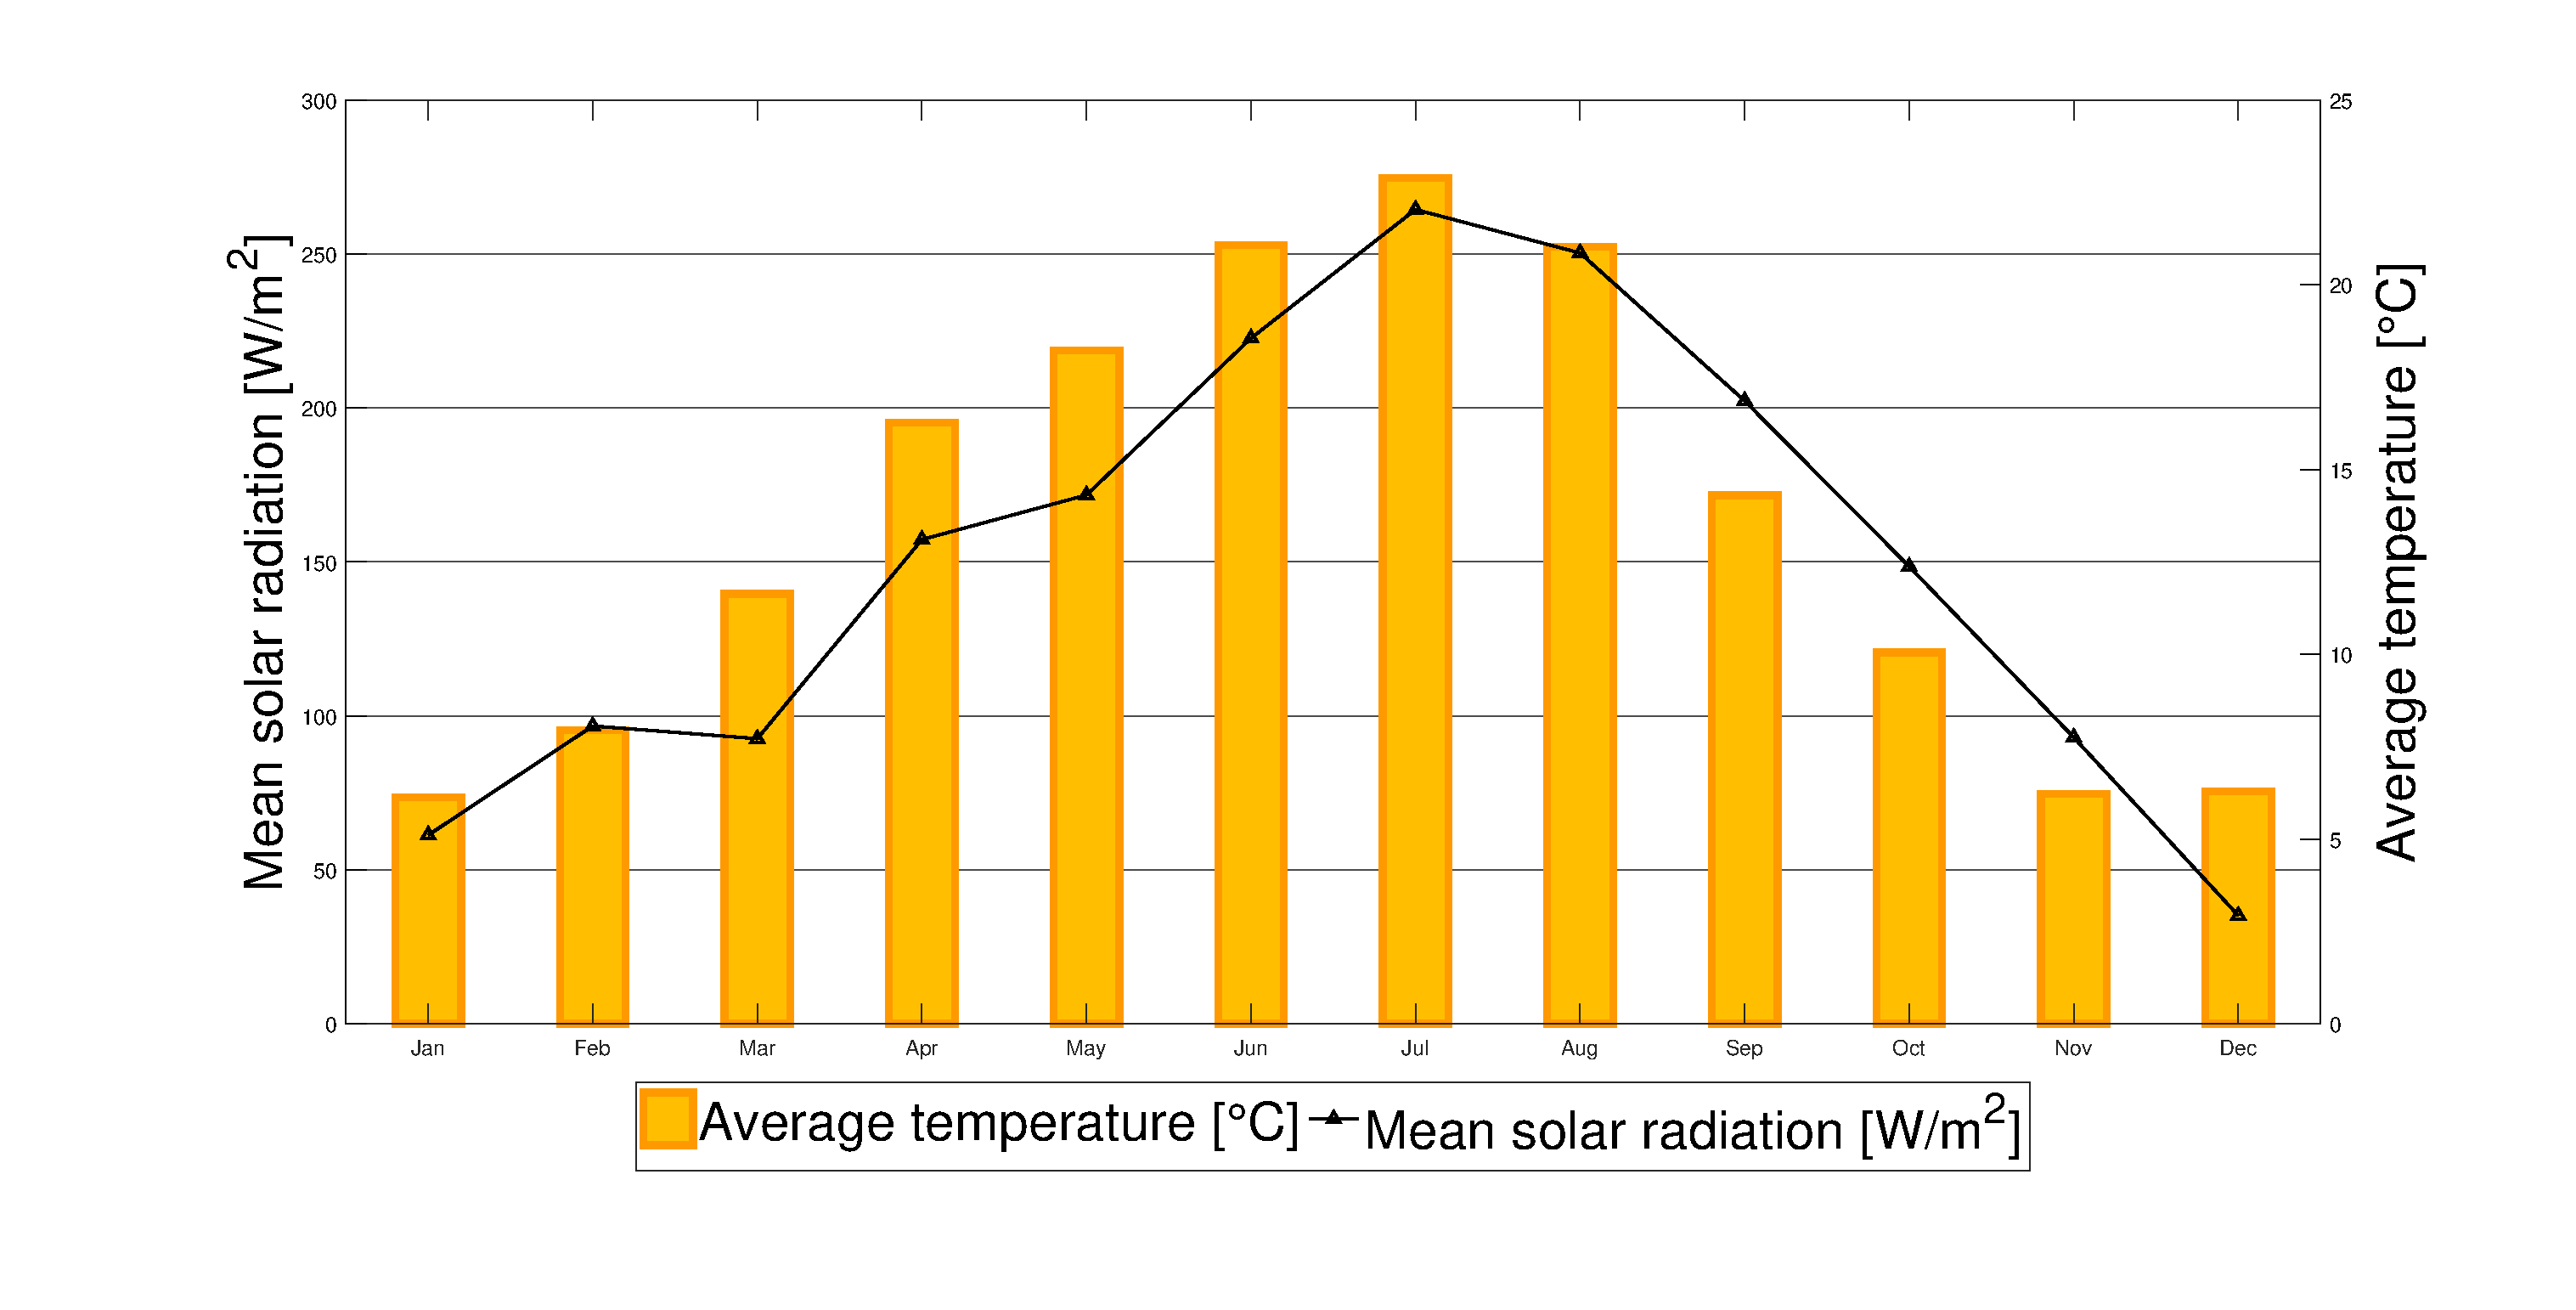
\includegraphics[width=26pc]{figures/dati_climatici_rev01.eps}
		\caption{Weather data of L'Aquila.}
		\captionsetup{justification=centering}
		\label{F:houseExternalWeather}
	\end{center}
\end{figure}

Because of the complex morphology of the blocks shown in Figure \ref{F:houseSection}, some simplified assumptions were made, in order to create the EnergyPlus virtual model. Considering the thermal properties of the wood-cement blocks that compose the walls shown in Figure \ref{F:houseSection1}, the thermal effects of the ribs were neglected. For the block employed for floor and roof shown in Figure \ref{F:houseSection2}, a less complex equivalent block, with only three layers, was evaluated in order to consider only one equivalent thermal transmittance value. The properties of the blocks used for the simulation model are listed in Table \ref{T:houseProperties}.    

\begin{table}[h!]
	\centering
	\begin{tabular}{ccccc}
		\toprule
		\multirow{3}{1.4cm}{\centering Structural member} & \multirow{3}{3.7cm}{\centering Layer description (from inside to outside)}     & Thermal     		    & Total     & Total        \\
		                                                  &                                                                                & resistance   		    & thickness & U-value      \\
		                                                  &                                                                                & $[(m^2K)/W]$		    & $[m]$     & $[W/(m^2K)]$ \\
		\midrule
		\multirow{3}*{Wall}                               & Wood-cement                                                                    & $0.308$     		    &           &              \\ 
		                            					  & Concrete                                                                       & $0.096$    		    & $0.50 $   & $0.12 $      \\ 
		                            					  & EPS and graphite                                                               & $6.774$    		    &           &              \\
														  &																				   &						&			&			   \\
		\multirow{3}*{Floor}        					  & Screed                                                                         & $0.027$     		    &           &              \\ 
							        					  & Polystyrene                                                                    & $6.000$     		    & $0.23 $   & $0.28 $      \\ 
							        					  & Wood-cement                                                                    & $0.308$     		    &           &              \\
														  &																				   &						&			&			   \\
		\multirow{5}{1.4cm}{\centering Pitched roof} 	  & \multirow{2}{3.7cm}{\centering Polyurethane resins and polyisocianurate foams} & \multirow{2}*{$4.000$} &           &              \\ 
														  &                                                                                &                        &           &              \\
														  & Screed                                                                         & $0.027$    		    & $0.31 $   &  $0.13 $     \\
							        					  & Polystyrene                                                                    & $6.000$    		    &           &              \\ 
							        					  & Wood-cement                                                                    & $0.308 $   		    &           &              \\
		\bottomrule
	\end{tabular}
	\caption{Wood-cement blocks properties.}
	\captionsetup{justification=centering}
	\label{T:houseProperties}
\end{table}

Therefore, the dynamic simulation model of the use case, shown in Figure \ref{F:houseVirtualModel}, has been created by analyzing the fundamental characteristics of the building (orientation, geometry, structural members, heating system components, air changes with natural ventilation, activity, internal gains, air leakages) and the weather file specifically created for L'Aquila. The comprehensive method was chosen for modeling the heating system, once checked all the characteristics of the components.

\begin{figure}[h!]
	\begin{center}
		\includegraphics[width=24pc]{figures/Render_rev01.eps}
		\caption{Virtual model of the use case.}
		\captionsetup{justification=centering}
		\label{F:houseVirtualModel}
	\end{center}
\end{figure}

In order to calibrate the EnergyPlus model, a comparison between simulated and measured thermal energy consumption was performed. Considering the off-grid characteristic of the house, the installation of a heat meter was necessary for acquiring the actual energy consumption. Moreover, the heat meter installation has allowed a detailed knowledge of the actual heating system scheduling, shown in Figure \ref{F:houseActualScheduling}, faithfully reproduced in the simulated model. The heat meter, that consists of two thermocouples for flow and return thermal fluid temperatures, a turbine flowmeter and a controller, employed Equation \eqref{Eq:energyConsumption} to calculate the real thermal energy consumption $\dot Q$ of the house.
\begin{equation}\label{Eq:energyConsumption}
\dot Q = 0.2777698\times10^{-3}\times\rho\times\Delta V\times c_p\times\Delta T
\end{equation}
In \eqref{Eq:energyConsumption} $\dot Q$ is the thermal energy consumption $[Wh]$, $\rho$ is the water density $[kg/m^3]$, $\Delta V$ is the water volume variation $[m^3]$ detected by the turbine flowmeter, $c_p = 4.186\, [kJ/(kgK)]$ is the water specific heat at constant pressure, $\Delta T$ is the difference between flow and return temperatures of the water $[K]$, $0.2777698∙10−3$ is a dimensionless conversion factor. The considered period goes from March $15^{th}$ $2016$ to April $15^{th}$ $2016$.

\begin{figure}[h!]
	\begin{center}
		\includegraphics[width=28pc]{figures/Scheduling_rev02.eps}
		\caption{Actual scheduling of the heating system, where white color means switched OFF and green color switched ON, and ($T_{ext,ave}$) is the external average temperature. From midnight to $8am$ the heating system is always switched off.)}
		\captionsetup{justification=centering}
		\label{F:houseActualScheduling}
	\end{center}
\end{figure}
Following the hourly calibration proposed by the M\&V guidelines of ASHRAE \cite{USDOE}, a simulated model is calibrated when the mean bias error (MBE) and the coefficient of variation of the root mean square error [CV(RMSE)] are less than acceptable tolerances, respectively equal to $\pm 10.0\%$ and $30.0\%$. MBE and CV(RMSE) have been calculated by using Equations \eqref{Eq:mbe} and \eqref{Eq:cvrmse}.

\begin{equation}\label{Eq:mbe}
MBE(\%) = \frac{\sum_{Period}{(S-M)_{Interval}}}{\sum_{Period}{M_{Interval}}} \times 100
\end{equation}

where $M$ is the measured $kWh$ and $S$ is the simulated $kWh$.

\begin{align}\label{Eq:cvrmse}
\nonumber CV(RMSE_{Period}) &= \frac{RMSE_{Period}}{A_{Period}} \times 100 \\
				            &= \sqrt{\frac{\sum{(S-M)^2_{Interval}}}{N_{Interval}}} \times \frac 1{A_{Period}} \times 100
\end{align}

where $A_{Period}$ is the mean of the measured data for the period, Equation \eqref{Eq:aperiod}, and $N_{Interval} = 4563$ is the number of time intervals in the monitoring period.

\begin{equation}\label{Eq:aperiod}
A_{Period} = \frac{\sum_{Period}{M_{Interval}}}{N_{Interval}}
\end{equation}

The comparison between numerical and experimental data is shown in Figure \ref{F:houseComparisonExperimental} and shows a quite good agreement. Therefore, with a MBE equal to $7.38\%$ and a CV(RMSE) equal to $8.37\%$, the EnergyPlus model of the use case can be considered well calibrated.  

\begin{figure}[h!]
	\begin{center}
		\subfigure[Thermal energy.]{
			\label{F:houseComparisonExperimentalEnergy}
			\centering
			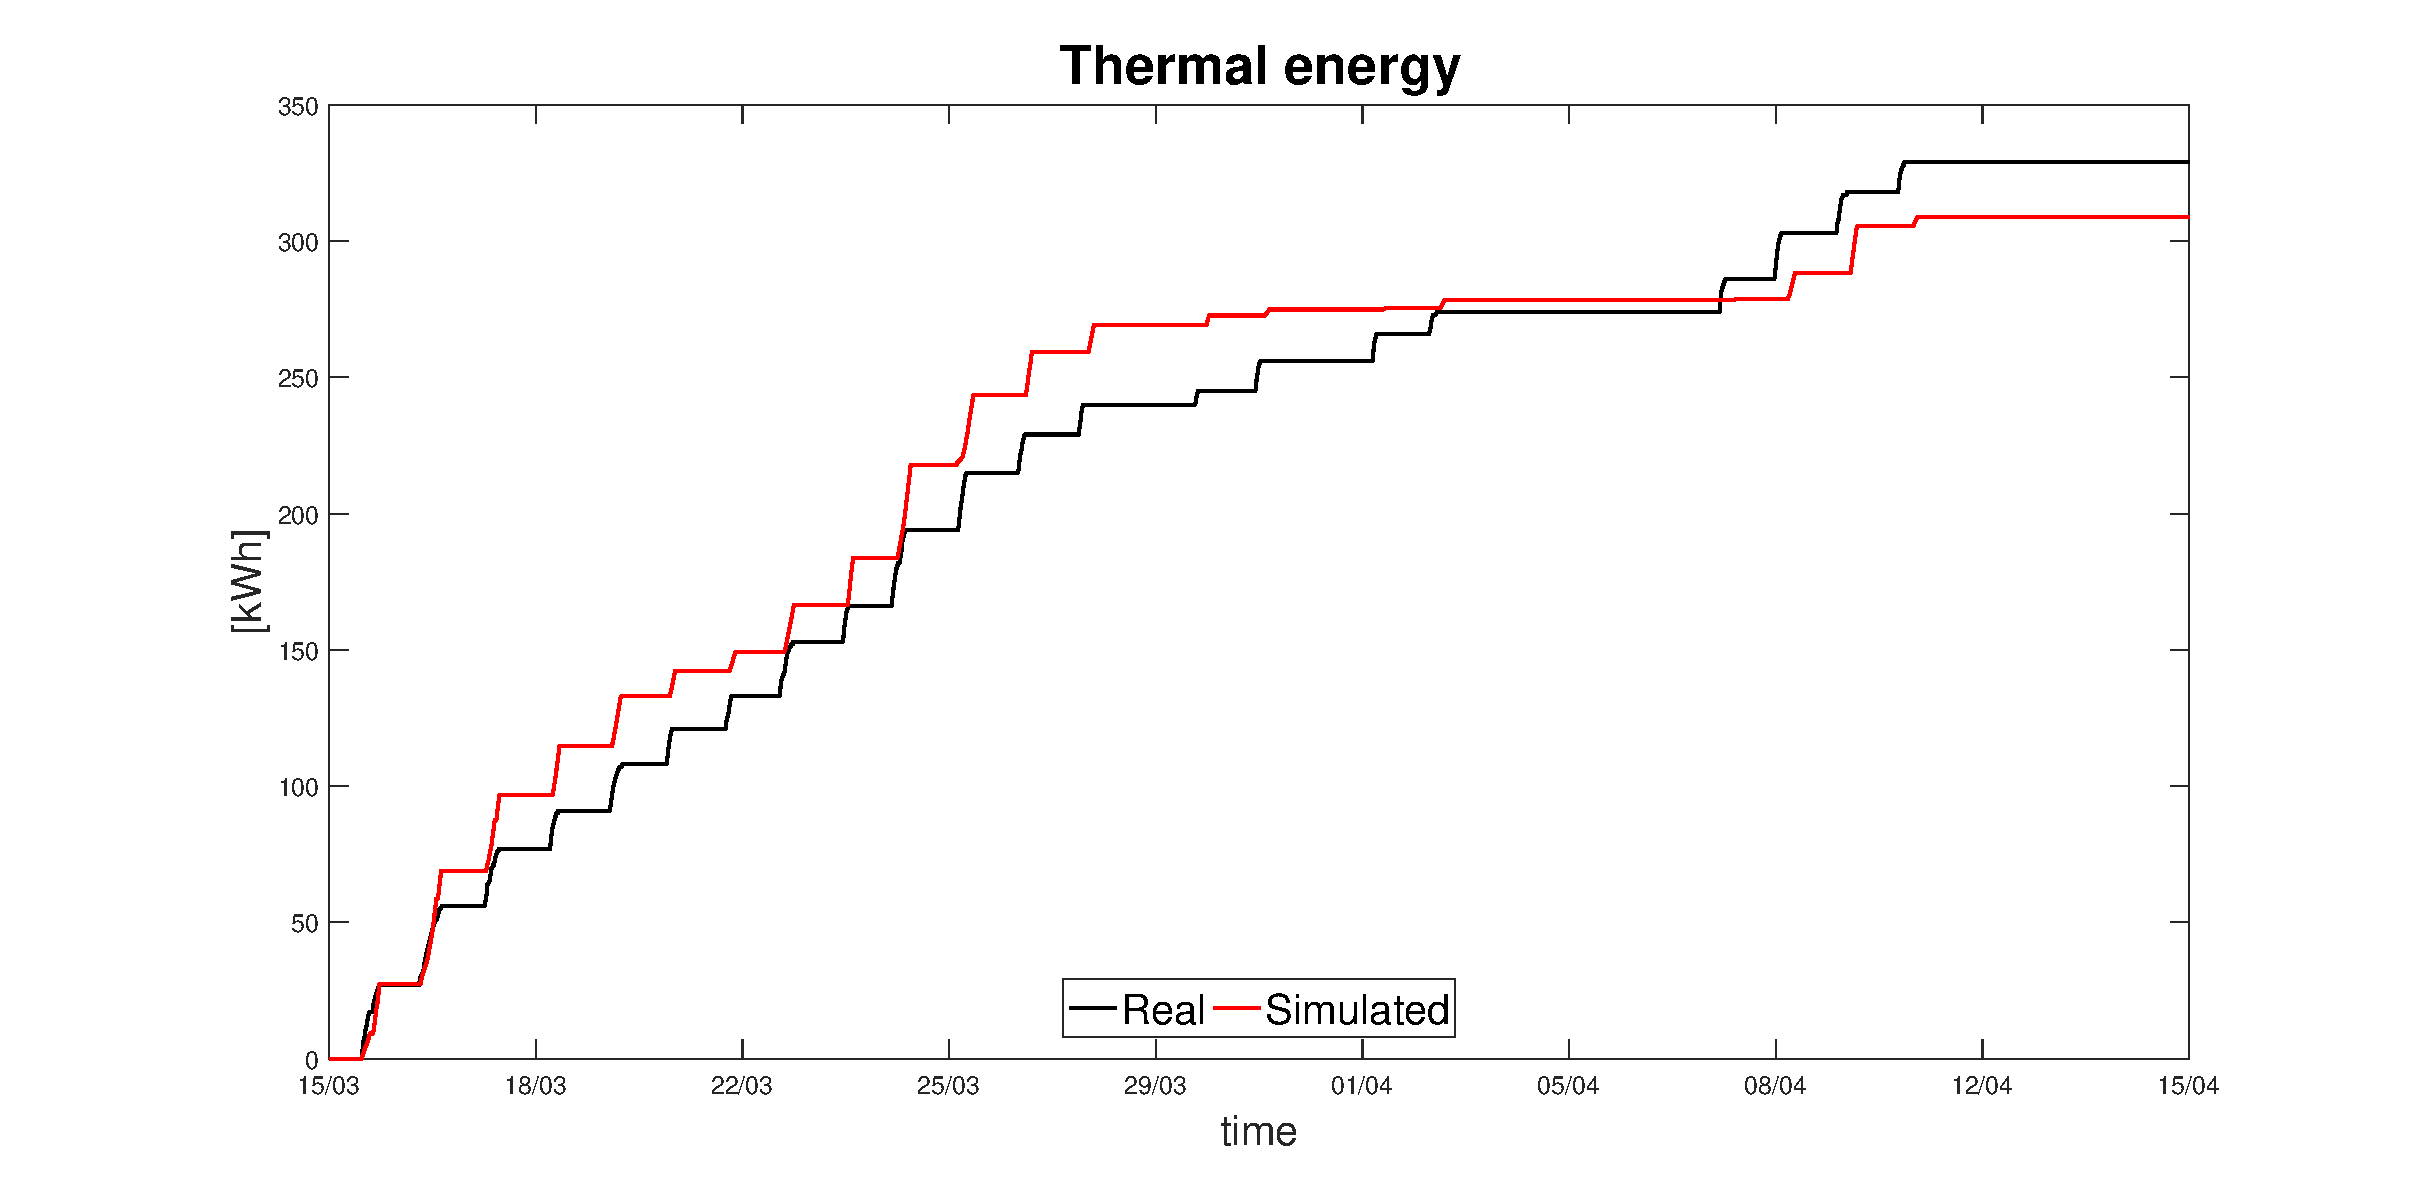
\includegraphics[width=24pc]{figures/Thermal_energy_rev01.eps}
		}
		\subfigure[Thermal power.]{
			\label{F:houseComparisonExperimentalPower}
			\centering
			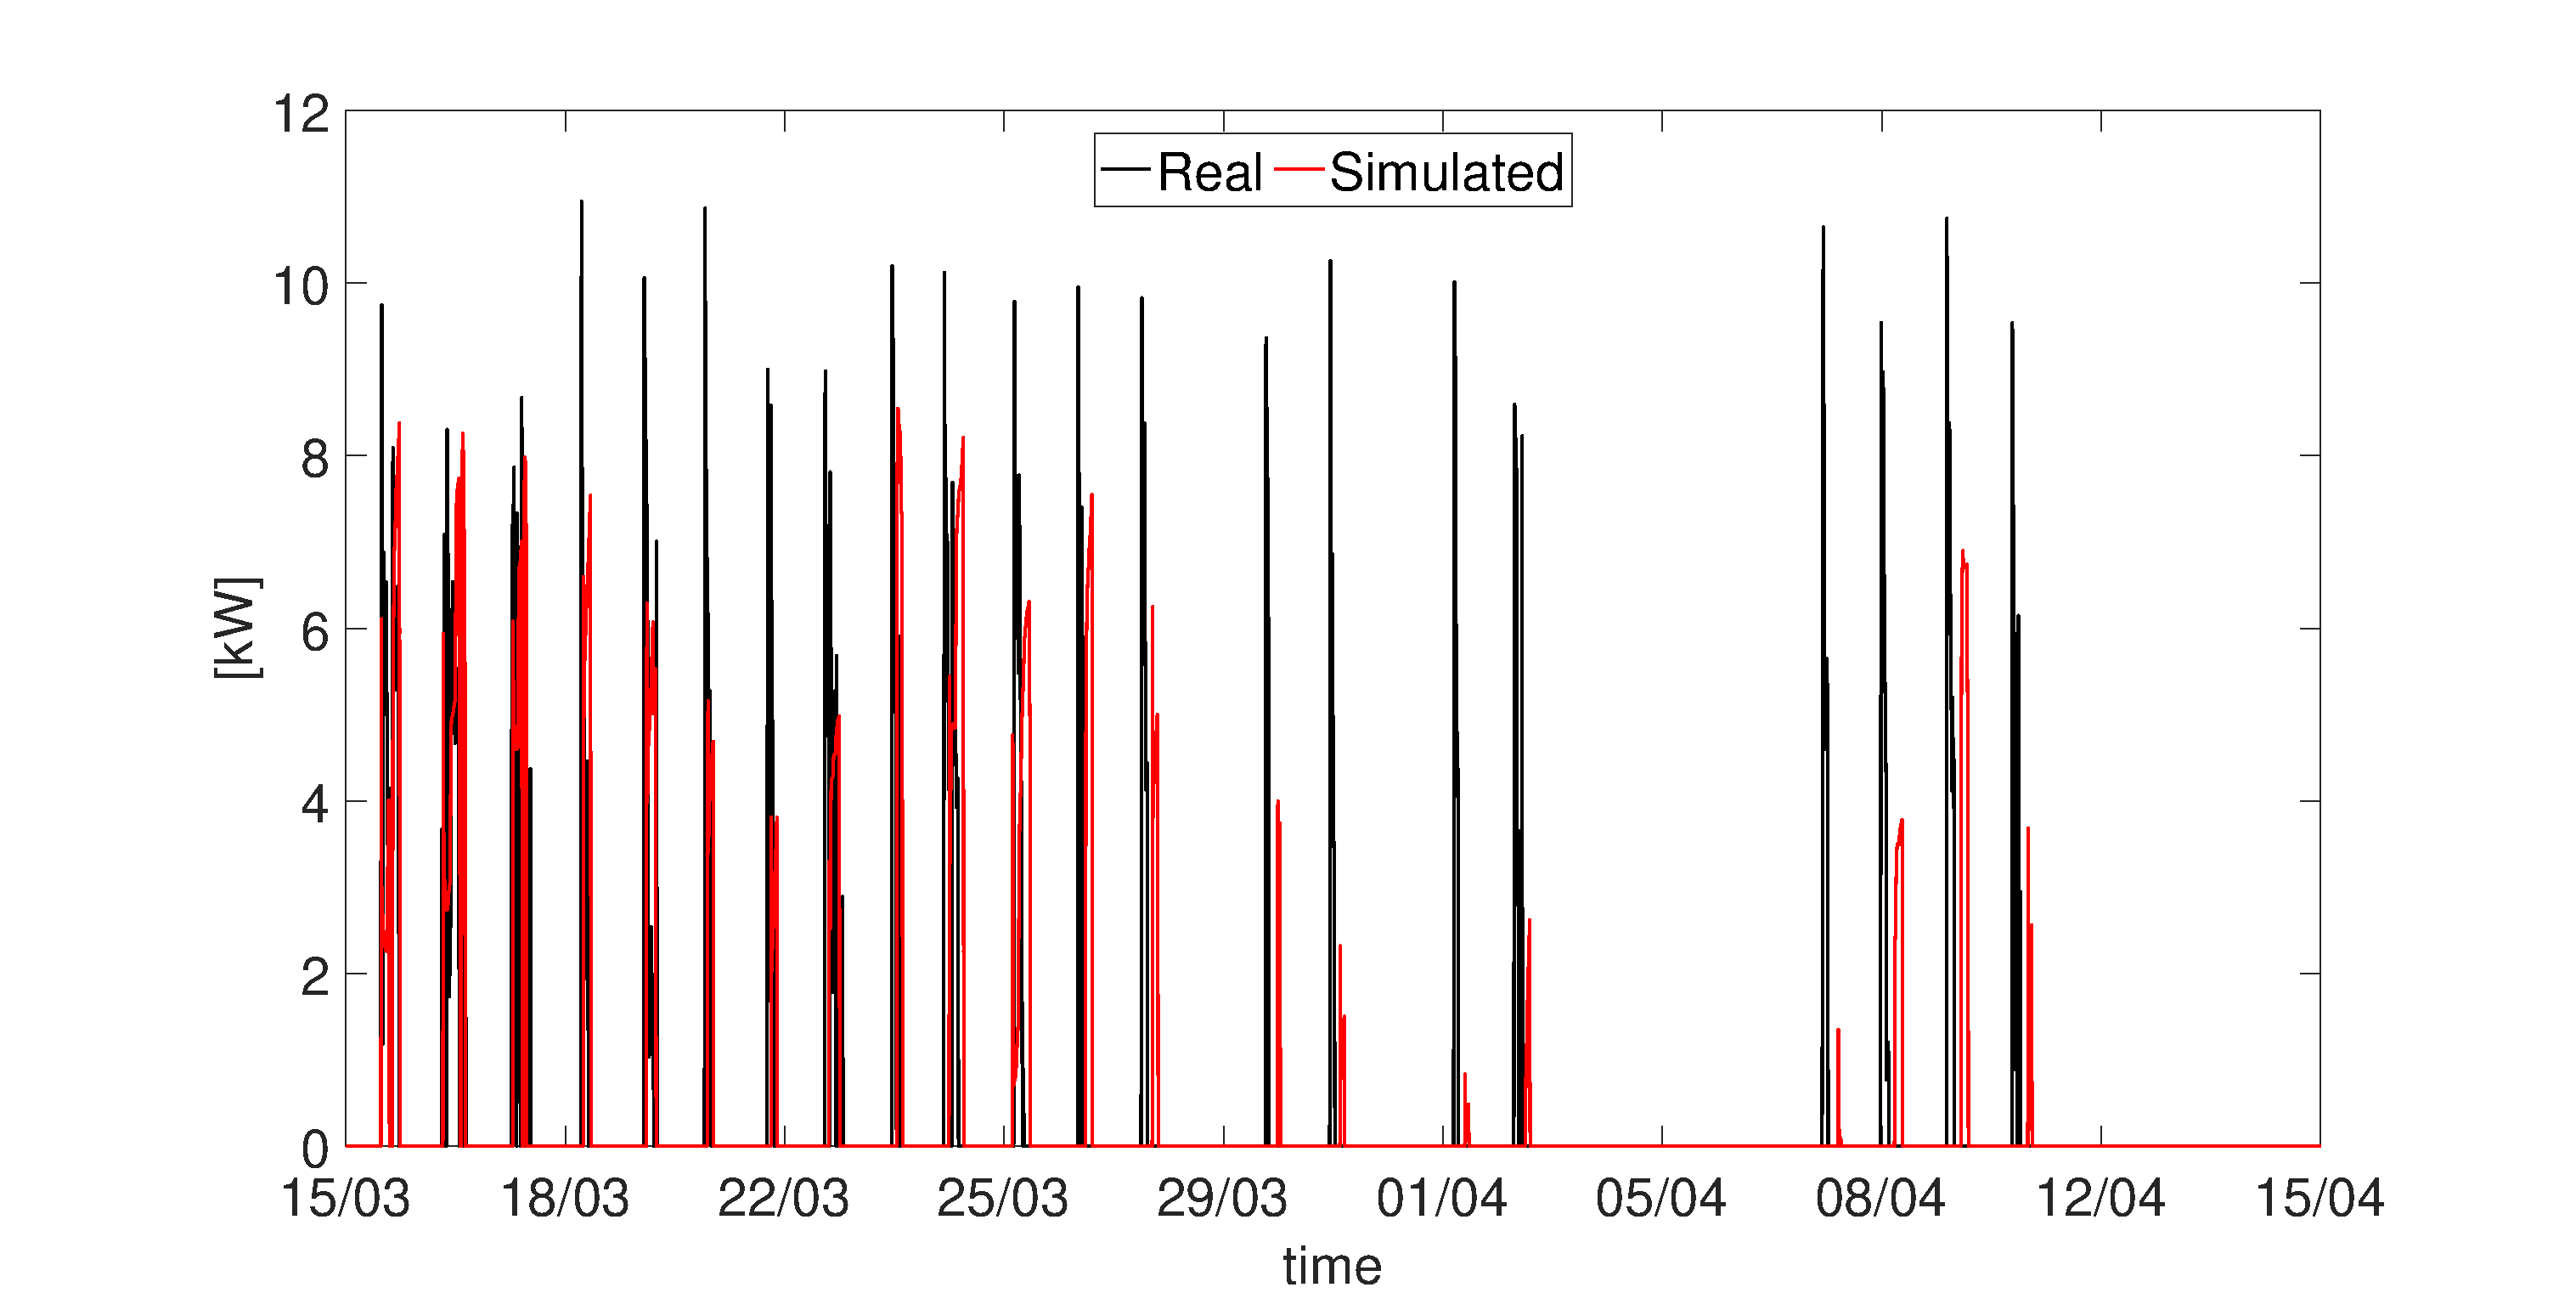
\includegraphics[width=24pc]{figures/Thermal_power.eps}
		}
	\end{center}
	\caption{Comparison between numerical and experimental data.}
	\captionsetup{justification=centering}
	\label{F:houseComparisonExperimental}
\end{figure}
\subsection{Random forest models} For the closed-loop simulations with DPC we create $2$ different sets of models, $S_1 = \{\tP^{r}_{\mathrm{k+1|k}},\tT^{r_1}_{\mathrm{k+1|k}},\tT^{r_2}_{\mathrm{k+1|k}},\tT^{r_3}_{\mathrm{k+1|k}},\tT^{r_4}_{\mathrm{k+j|k}}\}$ and $S_2 = \{\tP_{\mathrm{k+j|k}},\tT^{1}_{\mathrm{k+j|k}},\tT^{2}_{\mathrm{k+j|k}},\tT^{3}_{\mathrm{k+j|k}},\\\tT^{4}_{\mathrm{k+j|k}},\ j = 1,\ldots,N\}$, using random forests. In each set we have a model for the power consumption of the house ($\tP^{r}$ and $\tP$) and $4$ models that describe the evolution of the room temperature in each of the $4$ rooms ($\tT^{r_i}$ and $\tT^i$). Models in $S_1$ are created using the classical random forests algorithm with all the features and are used as plant simulator of the house. For this reason, they are computed to give prediction only for time step $k+1$ and not over the whole horizon $N$. Models in $S_2$ are used as predictors over a horizon $N$ in the DPC algorithm and are then created using the methodology provided in Section \ref{SS:dpcrf}. The non-manipulated features in $\tX^d$ are the disturbance data (relative humidity, atmospheric pressure, outside air temperature, solar radiation, wind, time of the day and day of the week) and the states (temperature of the $4$ rooms). The manipulated feature in $\tX^c$ is the flow rate ($[m^3/h]$). All this features are used to create models in $S_1$ and the power model in $S_2$, while disturbance data, state temperature of room $i$ only and flow rate are used to identify $\hat{\Theta}^{T}_{\tT^i_j}$ for temperature models in $S_2$. All the models have been trained on the data from March $11^{th}$ $2016$ to April $26^{th}$ $2016$ and validated on the data from May $1^{st}$ $2016$ to May $15^{th}$ $2016$. The accuracy of these models with respect to real data is shown in Table \ref{T:S1accuracy}, based on the definition of Normalized Root Mean Square Error (NRMSE).

\begin{table}[h!]
	\centering
	\begin{tabular}{cccccc}
		\toprule
		Set       & Power   & T. room $1$ & T. room $2$ & T. room $3$ & T. room $4$  \\ 
		\midrule
		$S_1$     & $92.44$ & $96.58$     & $96.99$     & $97.21$     & $96.62$\\
		$S_2$     & $92.21$ & $97.38$     & $97.29$     & $96.93$     & $96.81$\\
		\bottomrule
	\end{tabular}
	\caption{Models accuracy for power and temperatures models in $S_1$ and $S_2$ expressed as $\mathrm{1-NRMSE}\,(\%)$.}
	\captionsetup{justification=centering}
	\label{T:S1accuracy}
\end{table}

A graphical comparison is shown in Figure \ref{F:power_testing} for the power consumption and Figure \ref{F:temperature_testing} for the temperature of room $1$. The plots for the other rooms are omitted since they are very similar.

\begin{figure}[h!]
\begin{center}
	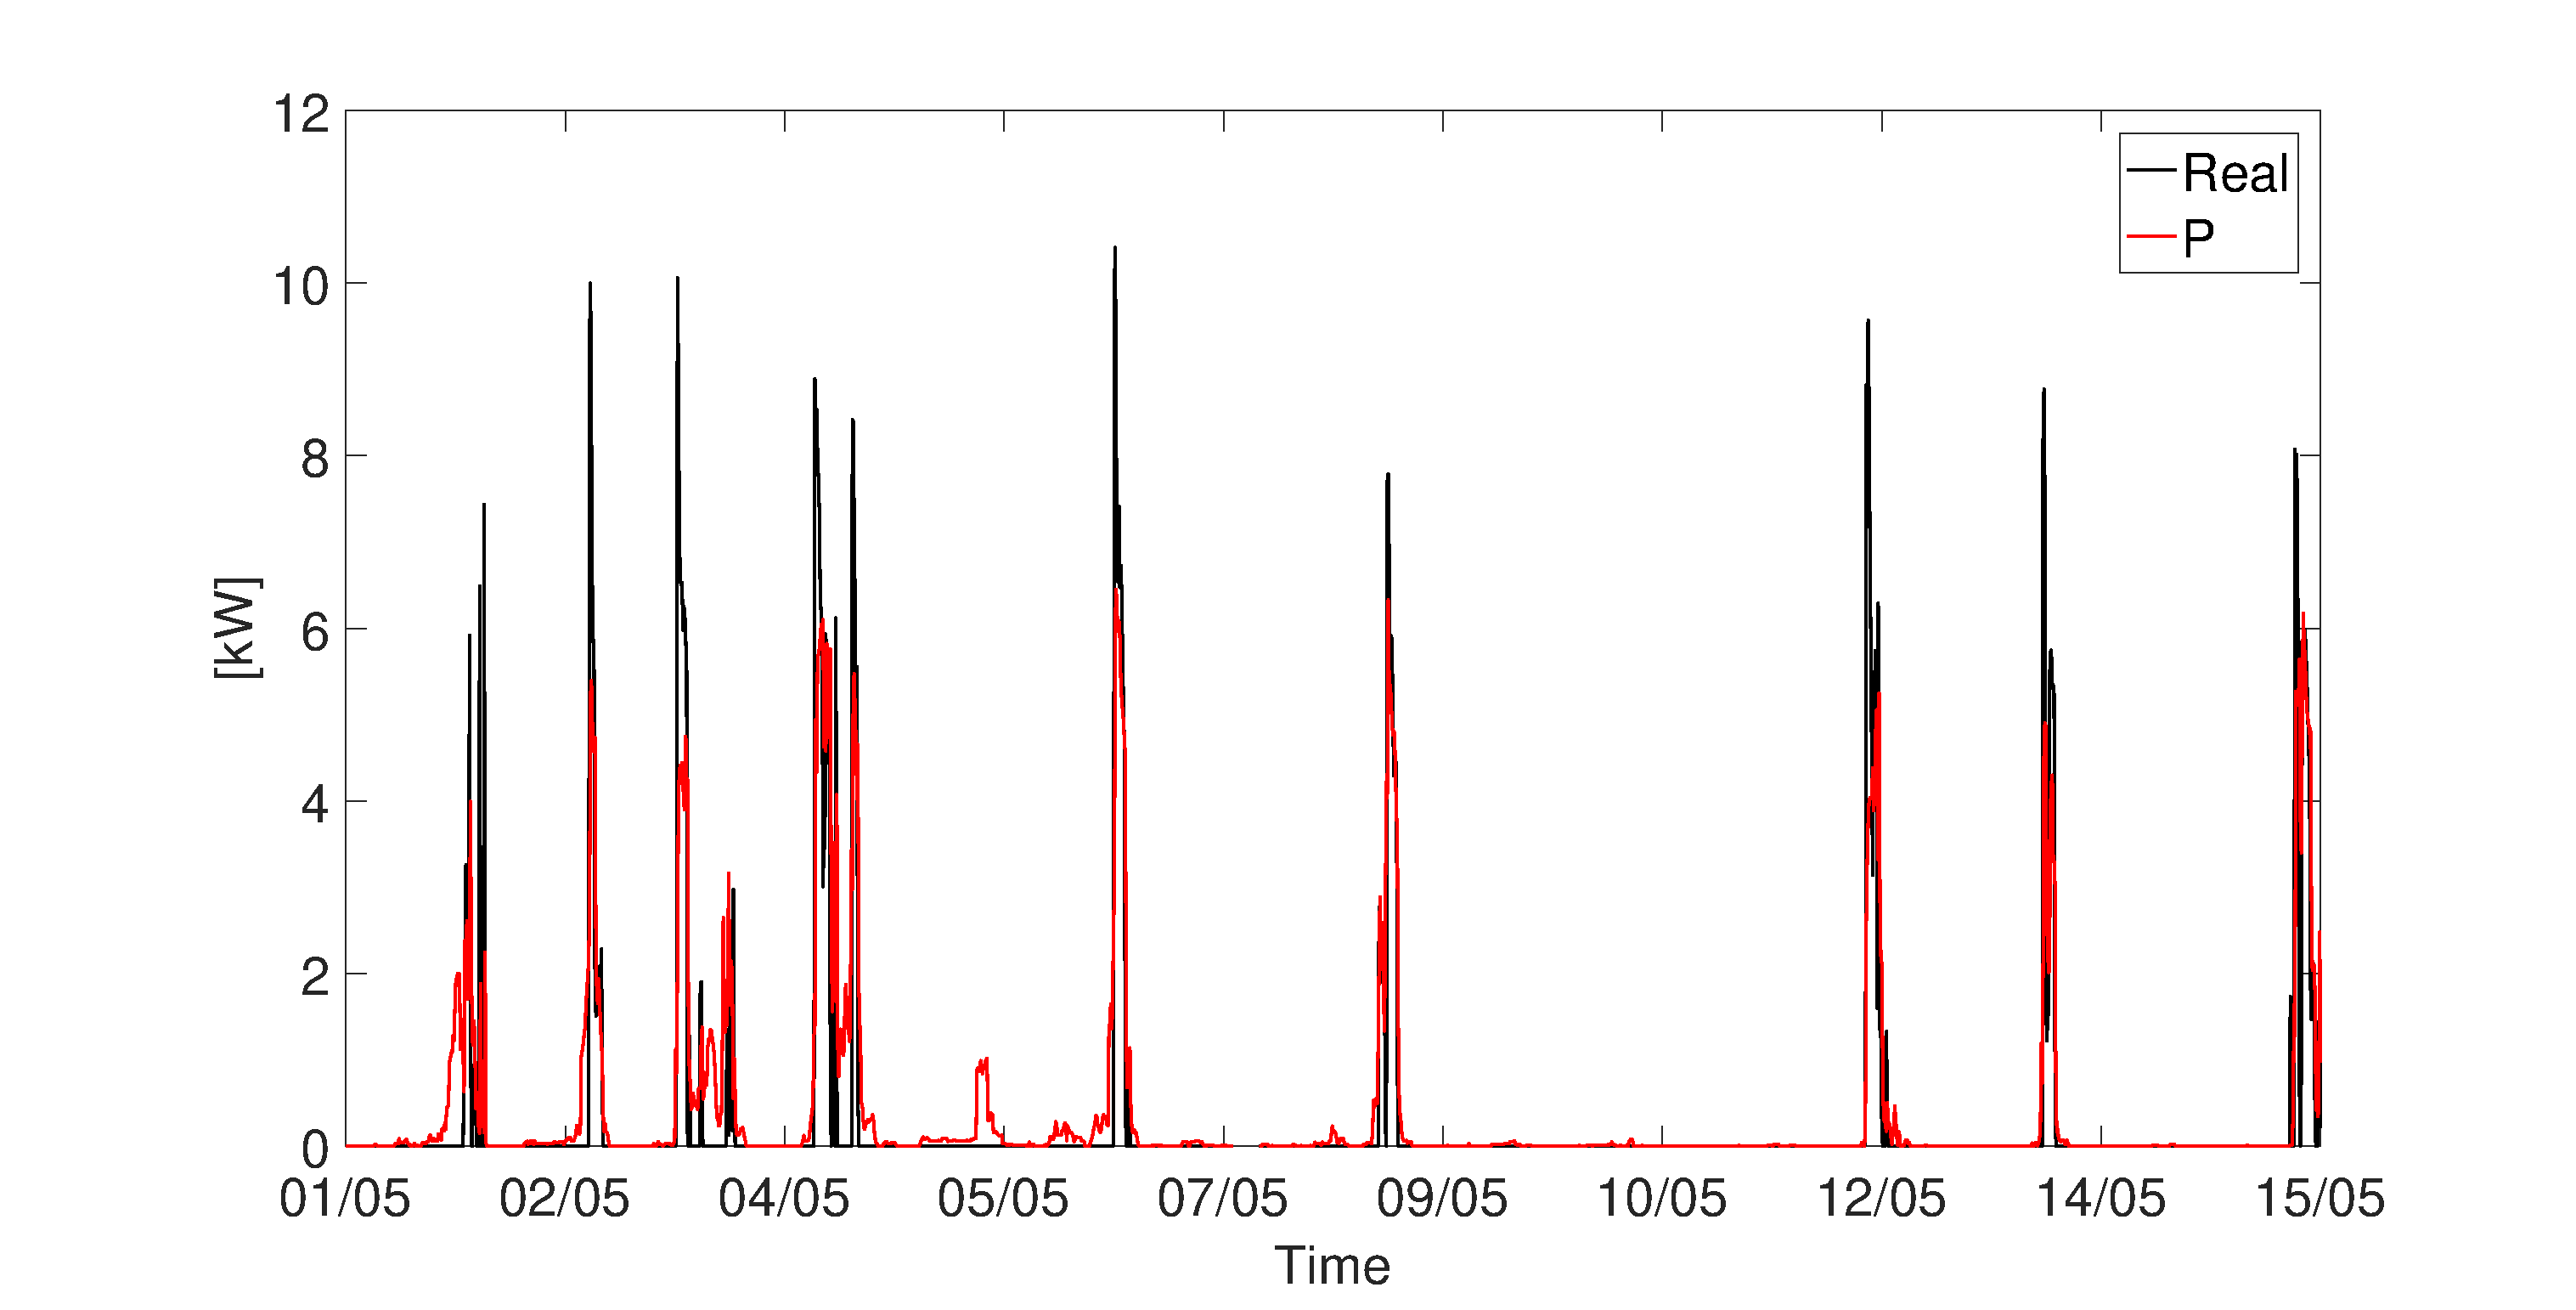
\includegraphics[width=26pc]{figures/power_testing.eps}
	\caption{Power consumption model accuracy validation.}
	\captionsetup{justification=centering}
	\label{F:power_testing}
\end{center}
\end{figure}

\begin{figure}[h!]
\begin{center}
	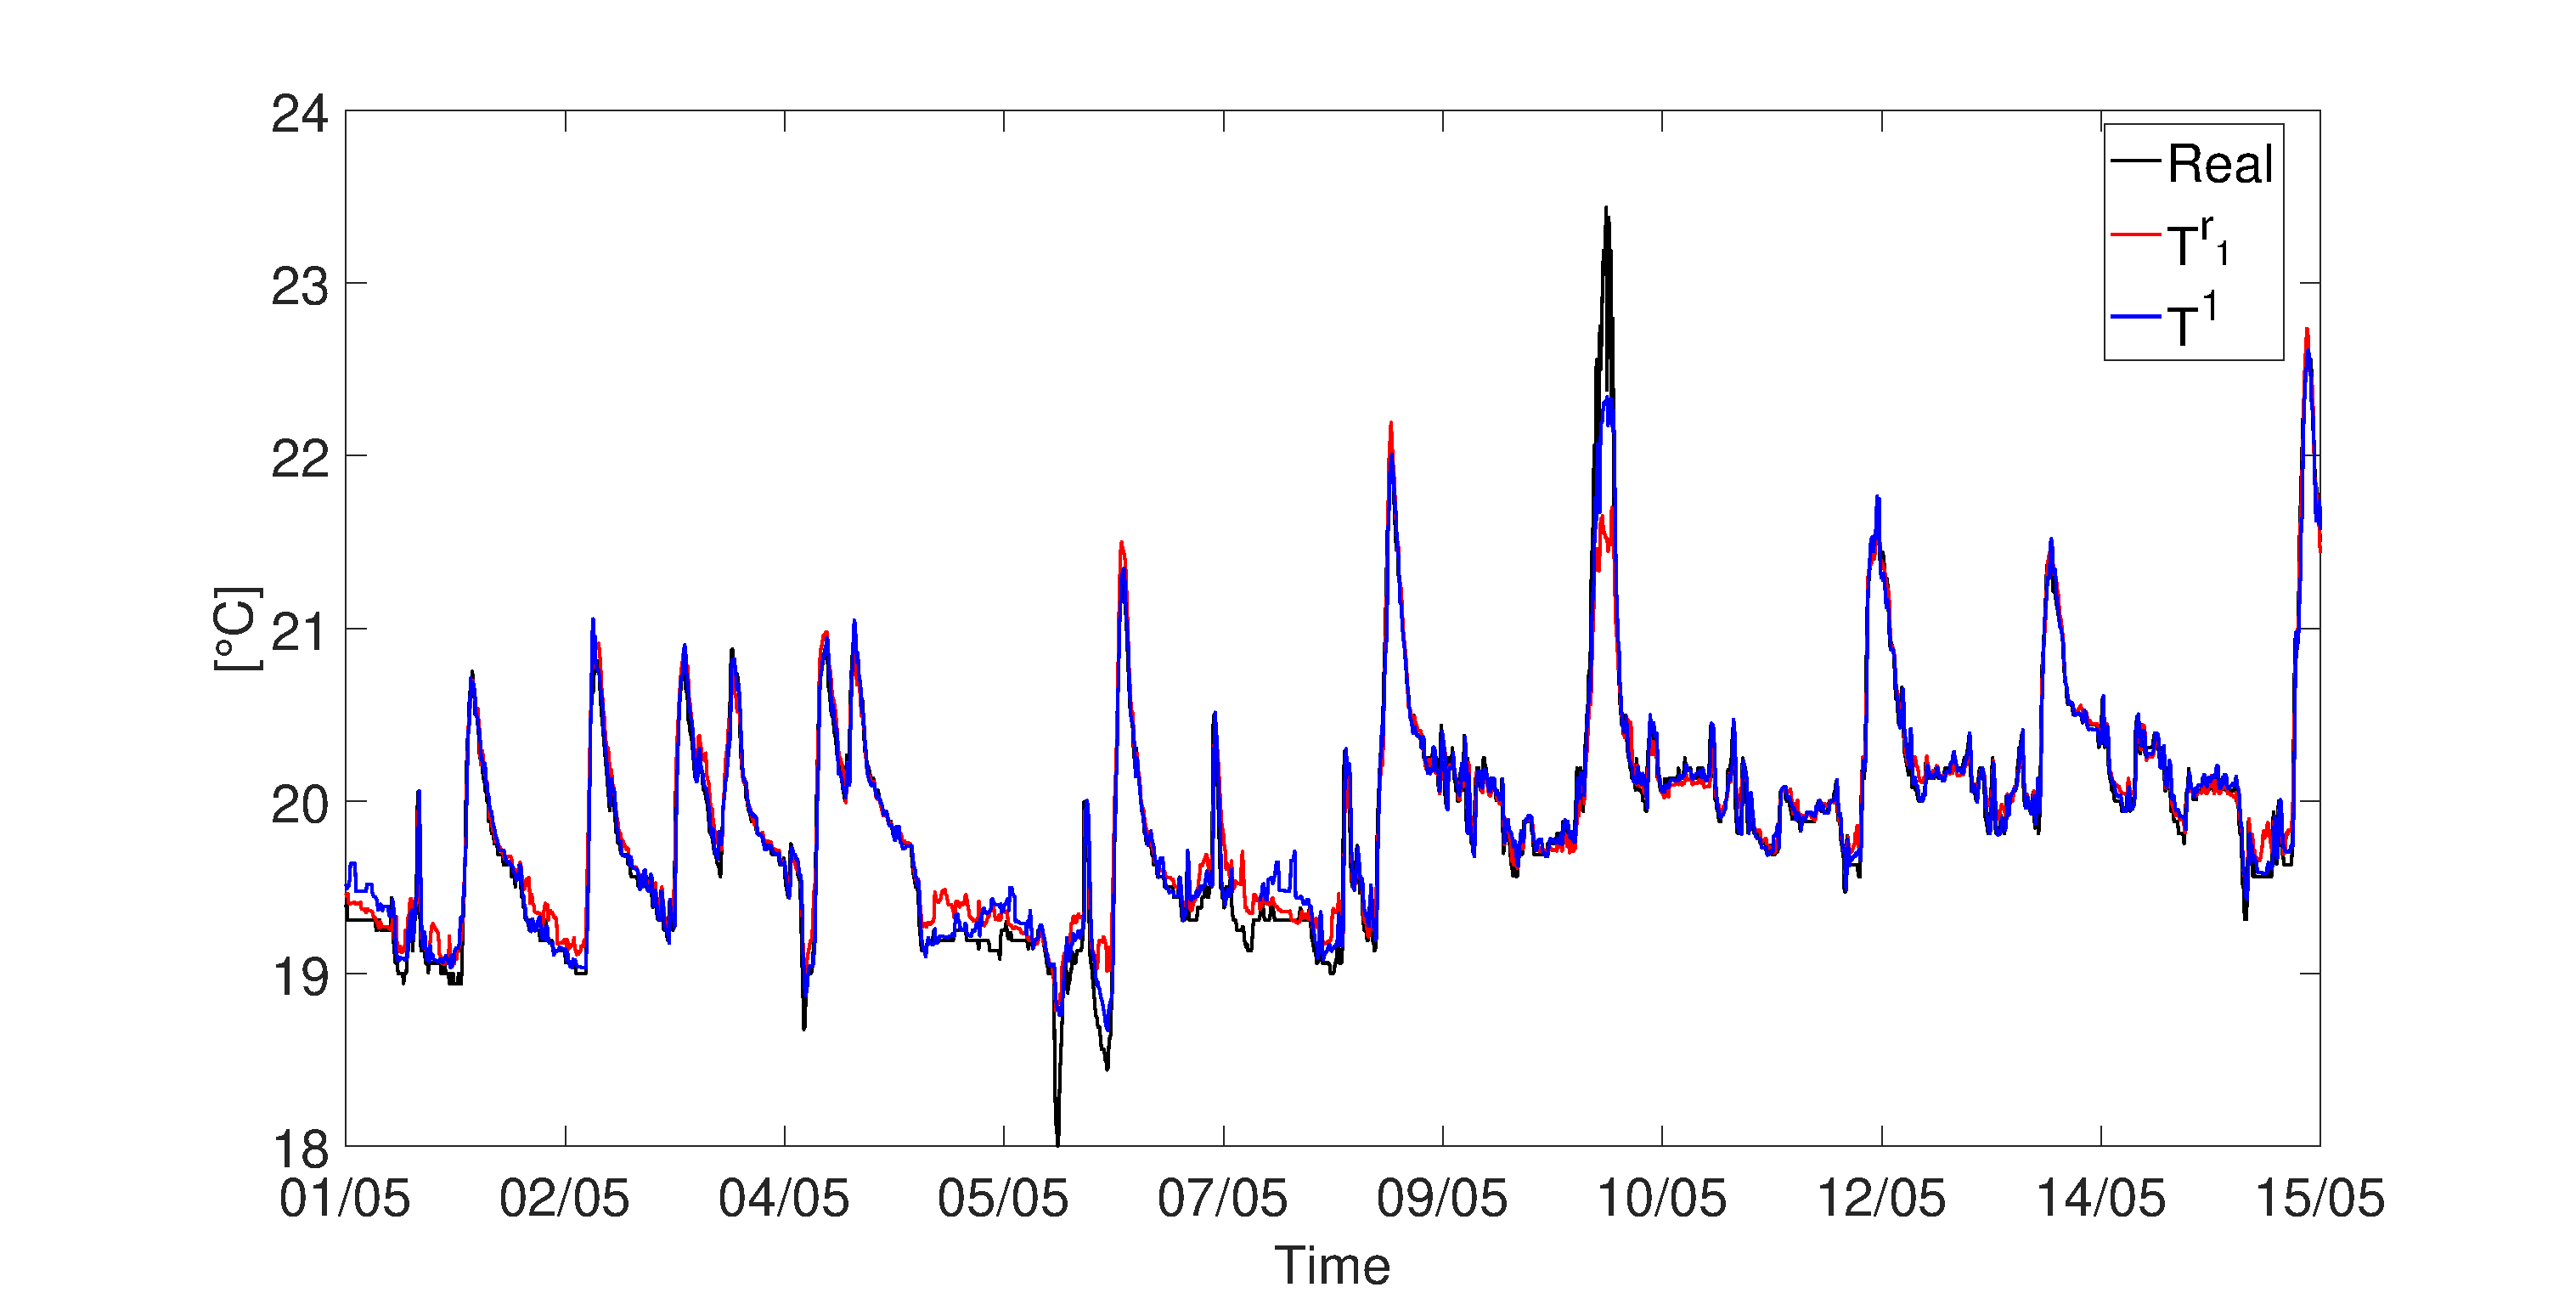
\includegraphics[width=26pc]{figures/temperature_testing.eps}
	\caption{Temperature model accuracy validation.}
	\captionsetup{justification=centering}
	\label{F:temperature_testing}
\end{center}
\end{figure}

We use random forest model $\tP^r$ also to estimate the energy consumption of the house. In particular we estimated it for the same period analyzed in Section \ref{SS:energyPlusmodel} and obtained the results in Figure \ref{F:Energy_testing}, with a MBE equal to $13.0\%$ and a CV(RMSE) equal to $13.7\%$.

\begin{figure}[h!]
	\begin{center}
		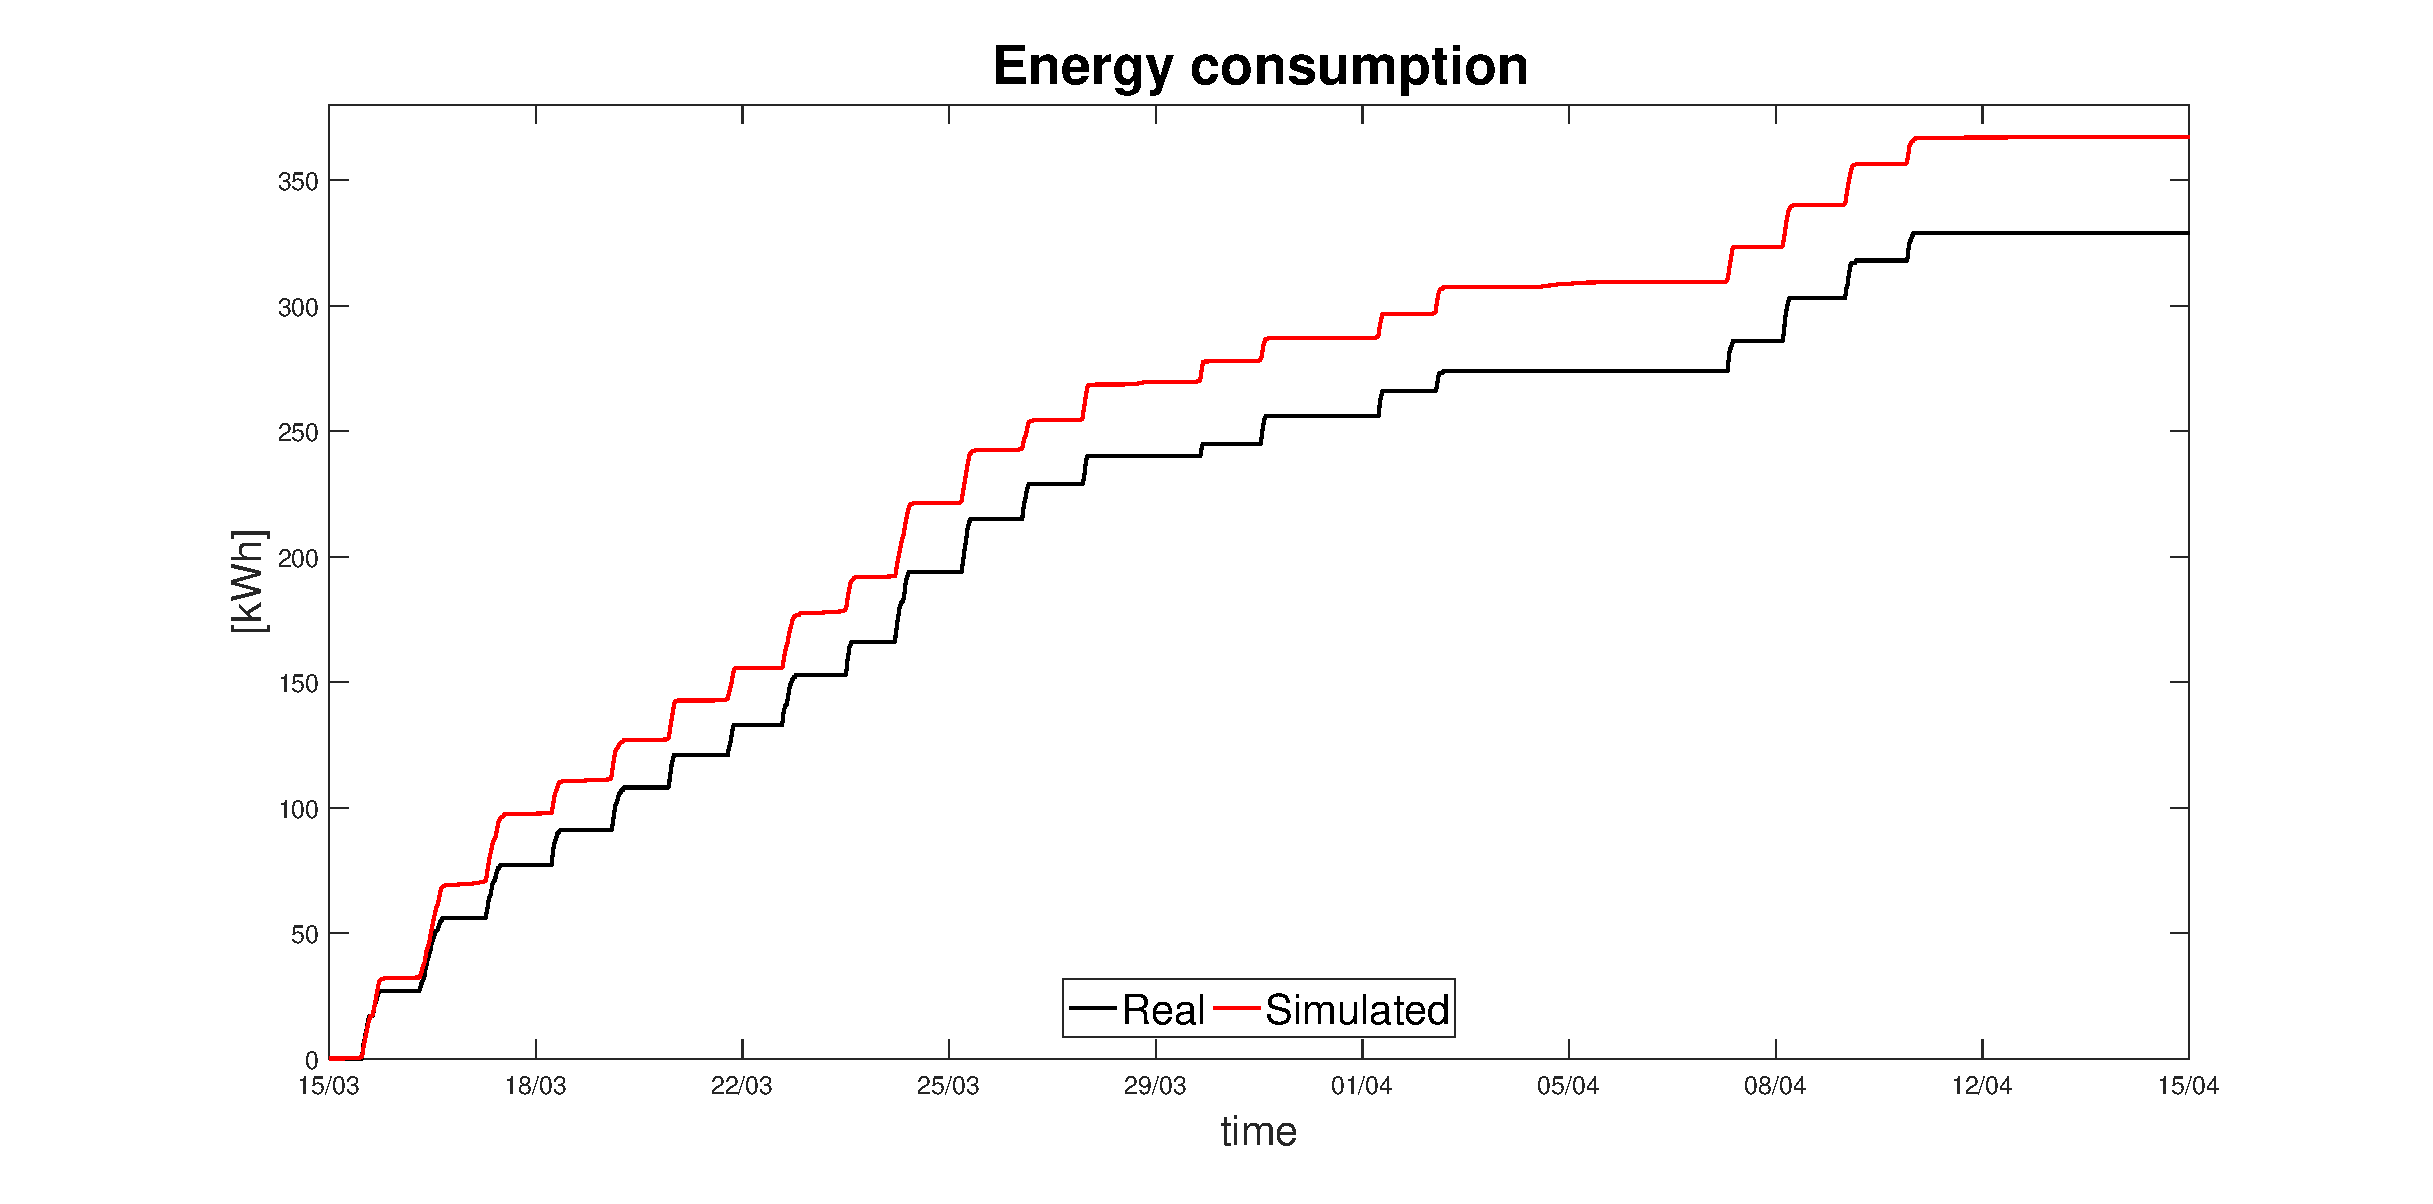
\includegraphics[width=26pc]{figures/Energy_test.eps}
		\caption{Energy consumption accuracy.}
		\captionsetup{justification=centering}
		\label{F:Energy_testing}
	\end{center}
\end{figure}

As we can see, with random forest model we get a worse MBE and CV(RMSE) for energy consumption, although the maximum error is very similar. This is because the EnergyPlus model, due to its internal dynamics based on the house structure, is able to compensate the error over time. On the other hand our curve perfectly follows the shape of the real case. For this reason, in Section \ref{SS:simulationResults}, we will use both models in order to compare the quality of the DPC with respect to a classical bang-bang controller.

\subsection{DPC and bang-bang controllers} We set up $2$ different controllers, DPC and bang-bang controller, to obtain a scheduling policy to switch the radiators ON and OFF in order to keep the temperature of room $3$ within a comfort range. Since the heating system serves all of the $4$ rooms simultaneously, without giving the possibility to control the temperature of each room independently, we setup the problem defining the comfort range only for one room. Other rooms temperatures will follow the scheduling policy. Room $3$ has been chosen randomly. In the following we describe the $2$ controllers.

\paragraph{DPC}
We want to optimize the ON/OFF heating system schedule in order to minimize power consumption of the house while keeping temperature of room $3$ within a comfort range. We also allow violations $\eps^{min},\eps^{max}$  of temperature bounds to guarantee feasibility of the algorithm. We include these violations in the objective function to be minimized. The problem is set up as follows:
\begin{align}
	\begin{aligned}
		\min_{\tX^c,\eps_j^{min},\eps_j^{max}} & \ \ \ \sum_{j=1}^{N} Q{\tP}_{\mathrm{k+j|k}}^2 +  \lambda_{min}\parallel\eps^{min}\parallel_2 + \lambda_{max}\parallel\eps^{max}\parallel_2 \\
		\text{s.~t. }& \ \ \ \ \ {\tP}_{\mathrm{k+j|k}} =  \hat{\Theta}^{T}_{\tP_j} [ 1,\tX^c_{\mathrm{k|k}},\dots,\tX^c_{\mathrm{k+j-1|k}} ]^T \\
					 & \ \ \ \ \ \tT^1_{\mathrm{k+j|k}} =  \hat{\Theta}^{T}_{\tT^1_j} [ 1,\tX^c_{\mathrm{k|k}},\dots,\tX^c_{\mathrm{k+j-1|k}} ]^T \\
					 & \ \ \ \ \ \tT^2_{\mathrm{k+j|k}} =  \hat{\Theta}^{T}_{\tT^2_j} [ 1,\tX^c_{\mathrm{k|k}},\dots,\tX^c_{\mathrm{k+j-1|k}} ]^T \\
			 	 	 & \ \ \ \ \ \tT^3_{\mathrm{k+j|k}} =  \hat{\Theta}^{T}_{\tT^3_j} [ 1,\tX^c_{\mathrm{k|k}},\dots,\tX^c_{\mathrm{k+j-1|k}} ]^T \\
				 	 & \ \ \ \ \ \tT^4_{\mathrm{k+j|k}} =  \hat{\Theta}^{T}_{\tT^4_j} [ 1,\tX^c_{\mathrm{k|k}},\dots,\tX^c_{\mathrm{k+j-1|k}} ]^T \\					
					 & \underline{\tT}_{\mathrm{k+j-1|k}}-\eps^{min}_j \leq \tT^3_{\mathrm{k+j|k}} \leq \overline{\tT}_{\mathrm{k+j-1|k}} + \eps^{max}_j\\
					 & \ \ \ \ \ \ \ \ \tX^c_{\mathrm{k+j-1|k}} = \underline{\tX}^c \lor \tX^c_{\mathrm{k+j-1|k}} = \overline{\tX}^c\\ 
					 & \ \ \ \ \ \ \ \ \,\eps^{min}_j,\eps^{max}_j \geq 0, \ j = 1,\dots,N.
	\end{aligned}
	\label{E:DPCrealcase}
\end{align}
The choice of different weights $Q$, $\lambda_{min}$ and $\lambda_{max}$ allows the designer to give more importance to energy consumption rather than temperature comfort and viceversa. In Section \ref{SS:simulationResults} we will show different performance results considering different weights. Parameters $\underline{\tX}^c$ and $\overline{\tX}^c$ are respectively minimum and maximum values the heating system can actuate, while $\underline{\tT}_{\mathrm{k+j-1|k}}$ and $\overline{\tT}_{\mathrm{k+j-1|k}}$ are respectively time varying lower and upper bounds to keep the temperature in a desired range of comfort. Due to the integer variable constraint for input $\tX^c$, the problem is a Mixed Integer Quadratic Programming. For the implementation we use in Section \ref{SS:simulationResults} Gurobi solver \cite{Gurobi2015} through CVX \cite{cvx,gb08}.

\paragraph{Bang-bang controller}
This is the classical controller widely used in private houses to keep temperature within a comfort range. It switches the heating system ON when the temperature goes under the temperature lower bound and switches it OFF when the temperature goes over the temperature upper bound. The advantage in using this controller is that it is very simple to set up. On the other hand it uses more energy than actually needed to achieve the task.

\subsection{Simulation Results}\label{SS:simulationResults} We simulated  DPC in \eqref{E:DPCrealcase} and the bang-bang controller, in closed-loop with the house models $\tT^{r_i}_{k+1|k},\ i=1,\ldots,4$ in $S_1$. We considered a sampling time of $10$ minutes and chose $N=4$ as a predictive horizon, i.e. $40$ minutes. From historical data we got that $\overline{\tX}^c = 0.35 \, m^3/h$ when the heating system is ON and obviously $\underline{\tX}^c = 0 \, m^3/h$ when the heating system is OFF. For the temperature comfort range we set a constant upper bound $\overline{\tT}_{\mathrm{k}} = 22.5 \, \degree C$ and a variable lower bound that is $\underline{\tT}_{\mathrm{k}} = 21 \, \degree C$ from $7am$ to $9am$, that is when people in the house wake up and go out for work, and from $6pm$ to midnight, that is when people come back from work and go to sleep, and $\underline{\tT}_{\mathrm{k}} = 20 \, \degree C$ during other hours, i.e. when people are either not home or sleep.

We said in Section \ref{SS:descriptionHouse} that the fuel used in the house is vegetable biomass. Therefore it is not possible to have ON/OFF switching phases too close to each other, differently from a traditional gas boiler, due to the burning process and heat exchange. For this reason we set up both control problems such that when the heating system is activated then it must stay active for at least $20$ minutes. This operating period can be obviously adapted depending on the fuel flow rate.

We ran DPC with $3$ different sets of parameters $Q$, $\lambda_{min}$ and $\lambda_{max}$. Each set allows a different level of temperature bounds violation. In particular we considered a small, a medium and a large violation configuration. The simulation period was from May $1^{st}$ $2016$ at $00am$ to May $5^{th}$ $2016$ at $1pm$.
\paragraph{Result 1} For the sake of clarity, we report in Figure \ref{F:comparison_small} only the comparison for temperature and input schedule obtained allowing small bound violations in DPC. We can see that the temperature controlled with DPC does not exit the bounds and if it does then it is around $0.1\,\degree C$. Bang-bang control also present small bounds violations due to its working principle. We can see how the DPC control law requires the heating system to be ON for less time than the bang-bang one to keep the temperature in the comfort range. We will see in Figure \ref{F:comparison_all_energy} that this translates in energy saving.

\begin{figure}[h!]
	\begin{center}
	\subfigure[Comparison of temperature of room $3$ obtained with DPC and bang-bang controller.]{
		\label{F:temperatures_small}
		\centering
		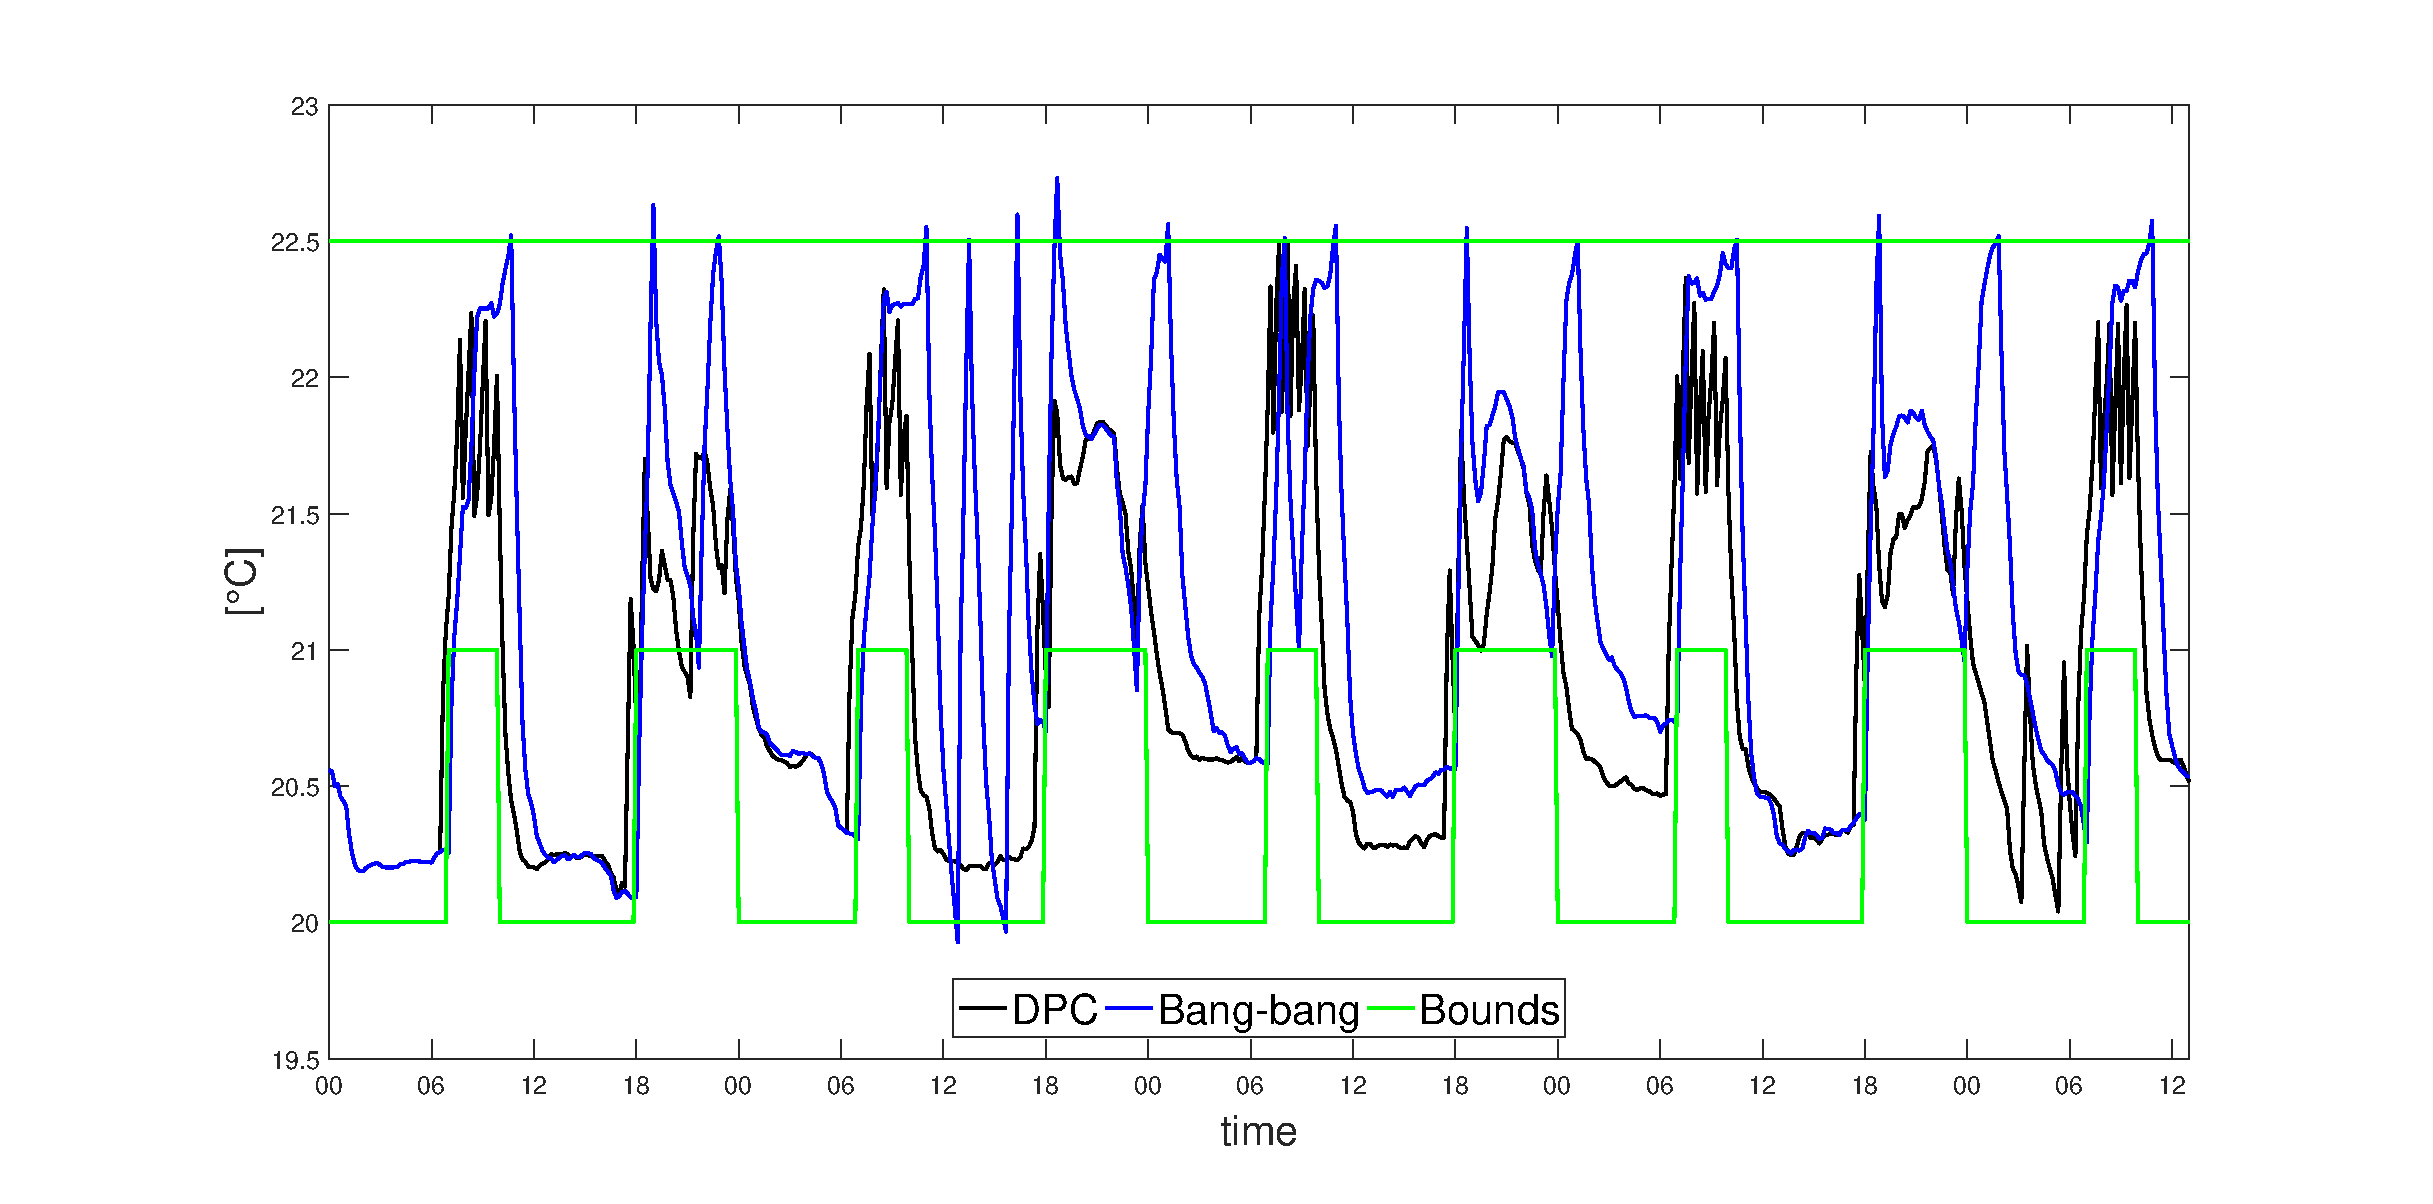
\includegraphics[width=26pc]{figures/Temperatures_small.eps}
	}
	\subfigure[Input schedules obtained from DPC and bang-bang controller.]{
		\label{F:inputs_small}
		\centering
		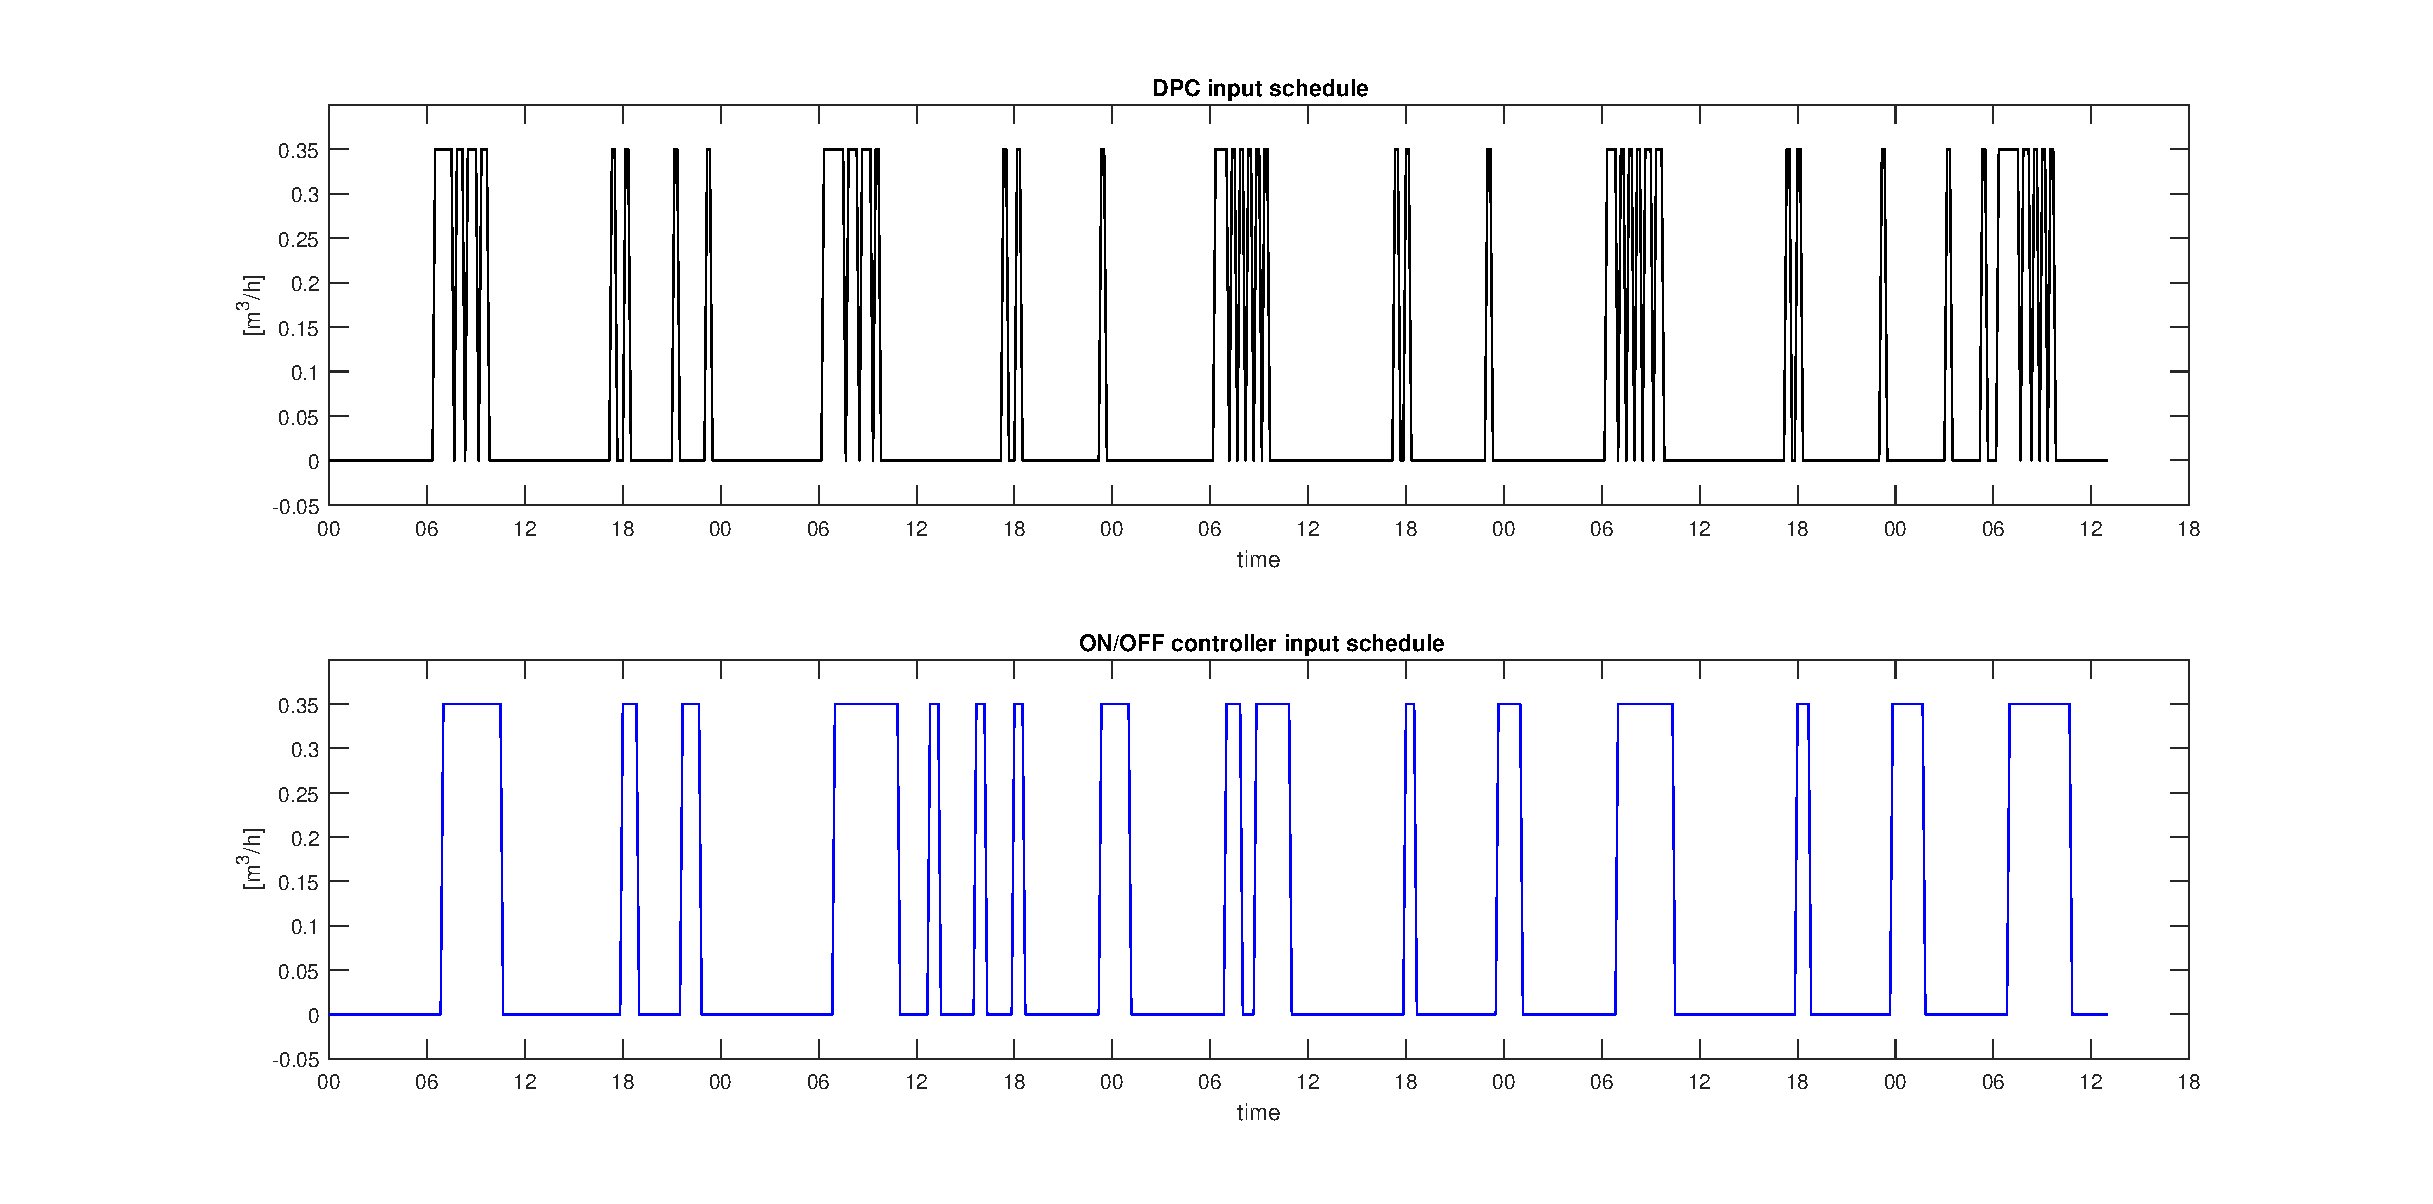
\includegraphics[width=26pc]{figures/Inputs_small.eps}
	}
	\end{center}
	\caption{Comparison of DPC and bang-bang control performance.}
	\captionsetup{justification=centering}
	\label{F:comparison_small}
\end{figure}

\paragraph{Result 2} In Figure \ref{F:comparison_all_temperature} a comparison of temperature regulation obtained running the DPC with small, medium and large violations is shown. The results show that with the large violation configuration, that gives more importance to the power consumption minimization than to keep temperature within the bounds, temperature is almost always outside the lower bound during the period when the range is tighter. However the maximum violation is still lower than $1\,\degree C$.
\begin{figure}[h!]
	\begin{center}
		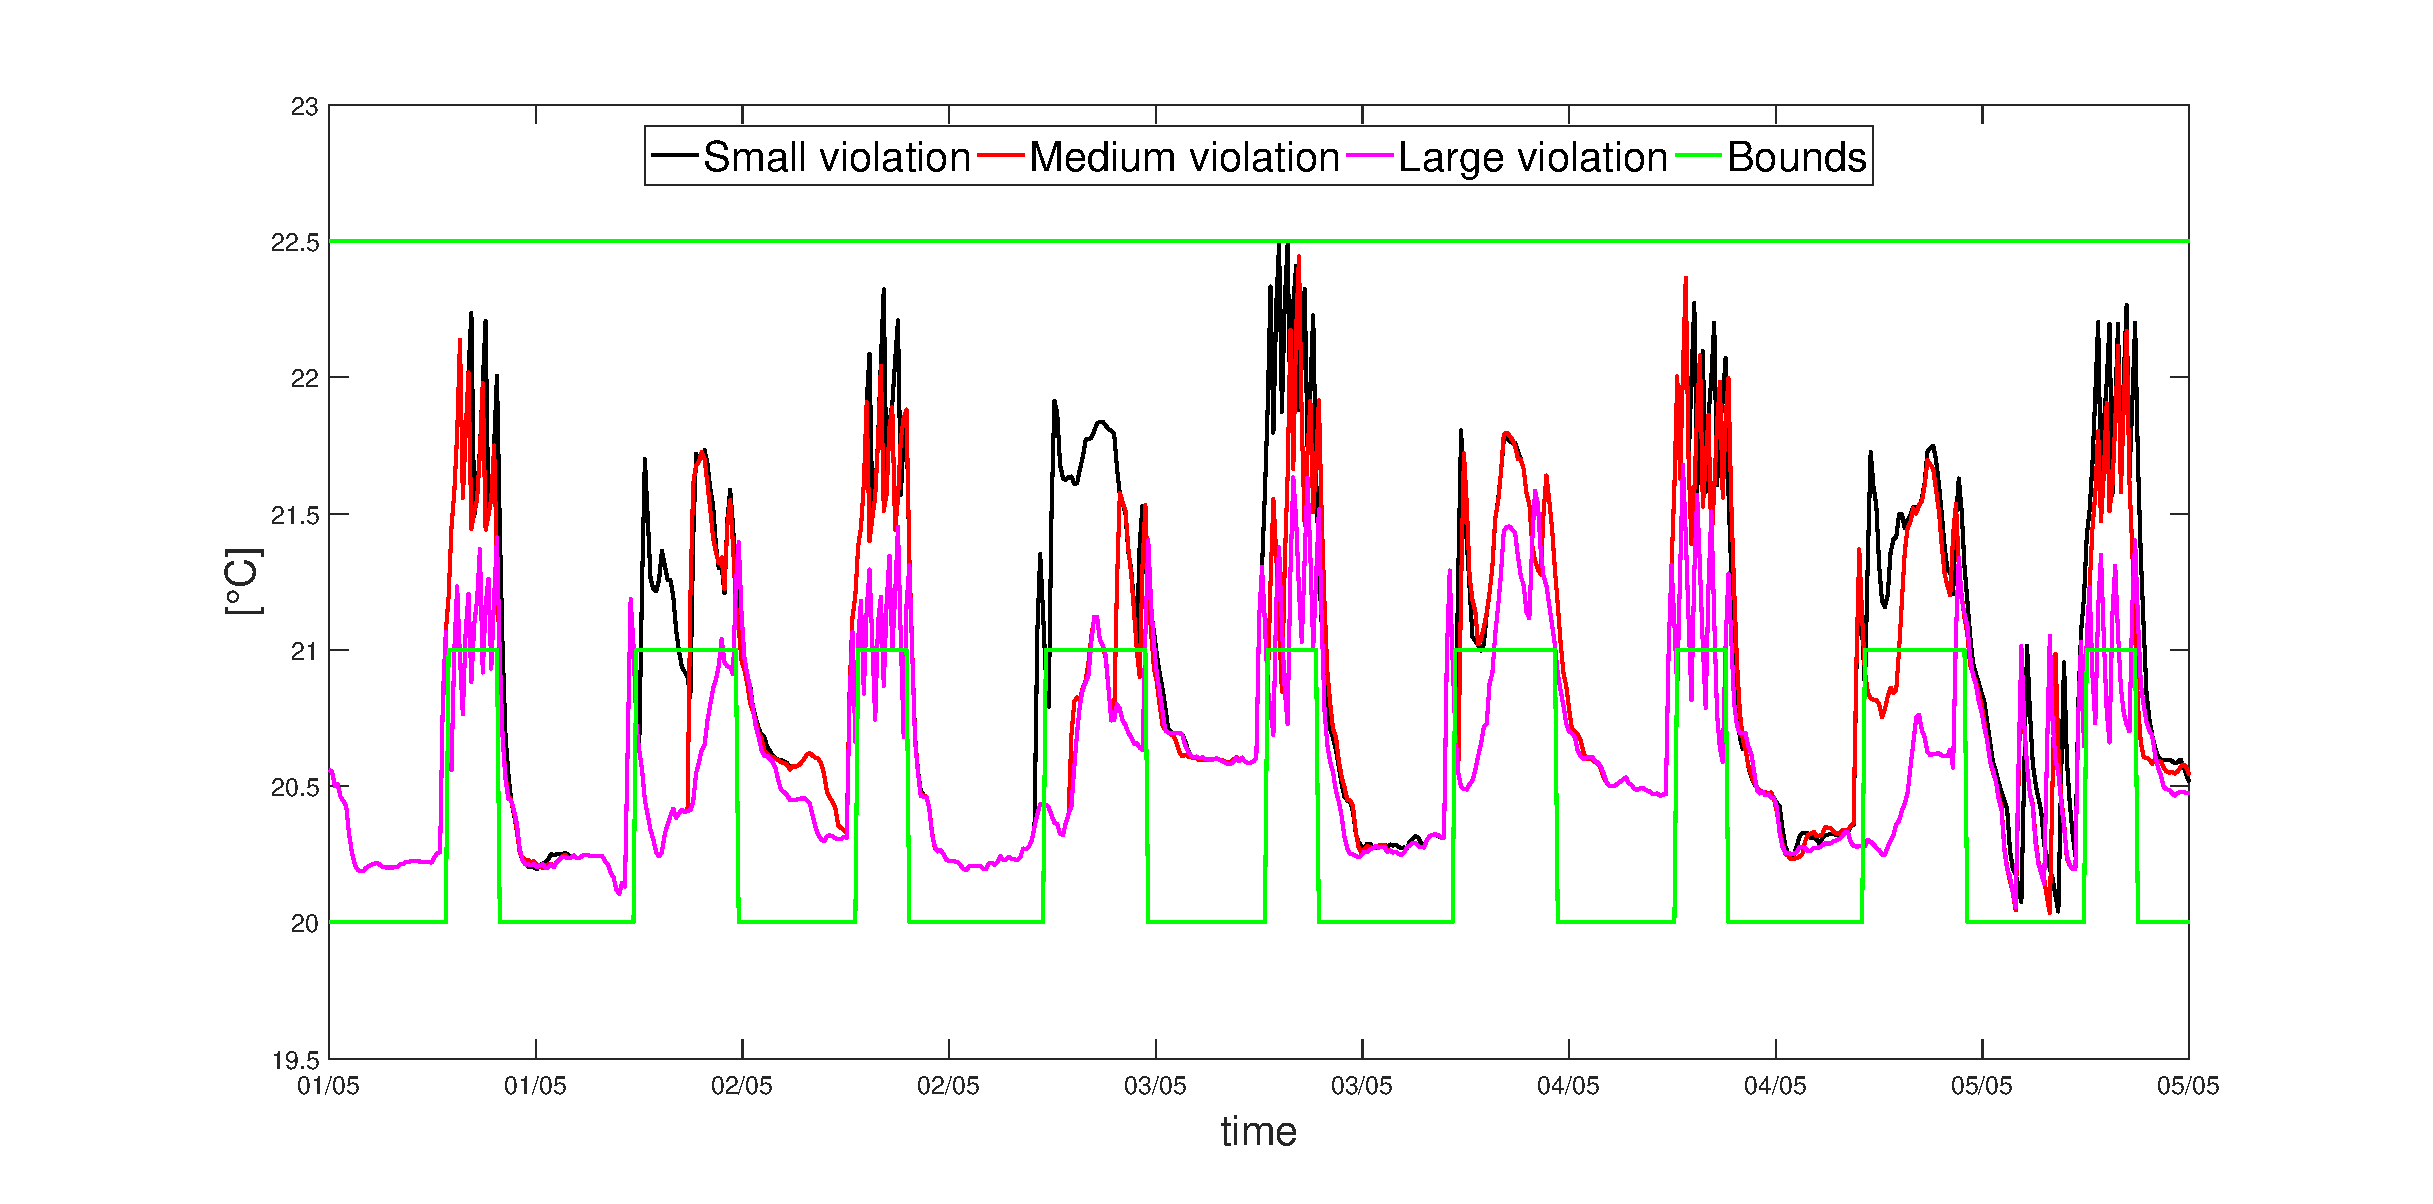
\includegraphics[width=26pc]{figures/Temperatures_all.eps}
	\end{center}
	\caption{Comparison of DPC control performance in terms of comfort with different violations.}
	\label{F:comparison_all_temperature}
\end{figure}
In Table \ref{T:violationErrors}, MBE and CV(RMSE) violation errors are reported to quantify the bounds violation of DPC, in each of the $3$ configurations, and of bang-bang controller.
\begin{table}[h!]
	\centering
%	\scalebox{0.9}{
		\begin{tabular}{cccccc}
			\toprule
			CONTROLLER  & LBV $\mathrm{MBE}$  & LBV $\mathrm{RMSE}$ & UBV $\mathrm{MBE}$ & UBV $\mathrm{RMSE}$ 	\\ 
			\midrule
			$DPC-SV$    & $0.013$             & $0.028$  			      & $0$    				 & $0$     	  	\\
			$DPC-MV$    & $0.165$ 			  & $0.146$     			  & $0$    				 & $0$		  	\\
			$DPC-LV$    & $0.410$  			  & $0.224$     			  & $0$    				 & $0$	      	\\
			$Bang-bang$ & $0.049$ 			  & $0.080$    				  & $0.0063$ 		     & $0.0120$	  	\\
			\bottomrule
		\end{tabular}
%	}
	\caption{Lower Bound Violation (LBV) and Upper Bound Violation (UBV) errors expressed as $\mathrm{MBE}\%$ and $\mathrm{CV(RMSE)}\%$ for DPC Small Violation (DPC-SV), DPC Medium Violation (DPC-MV), DPC large Violation (DPC-LV) and bang-bang controller.}
	\captionsetup{justification=centering}
	\label{T:violationErrors}
\end{table}
We can see that if we allow very small violations, DPC outperforms bang-bang controller in terms of comfort guarantees.

\paragraph{Result 3} In Figure \ref{F:comparison_all_energy}, using the neregy model derived from random forest power model $\tP^r$, we show how DPC outperforms the bang-bang controller also in terms of energy consumption and how the bounds violations allows us to save more energy. We can see that if we want to keep the temperature within a comfort range, only allowing small violations, the use of DPC produce an energy saving of $44\, kWh$, that correspond to the $33.0\%$ over a period of $4$ days and a half. Instead if we allow a large violation over the same period, the energy saving is of $78\, kWh$, that correspond to the $59.0\%$. If we consider these results over a monthly period, i.e. multiplying them for $6$, we get a monthly energy saving that goes from $264\,kWh$ to $468\,kWh$, with different comfort constraint configurations. Considering that the equivalent price of $1\,kWh$ of vegetable biomass is $TOT$\euro{} (TULLIO MAY YOU TELL ME ABOUT THIS PART?), we have a monthly saving of $TOT$\euro{}.

\begin{figure}[h!]
	\begin{center}
		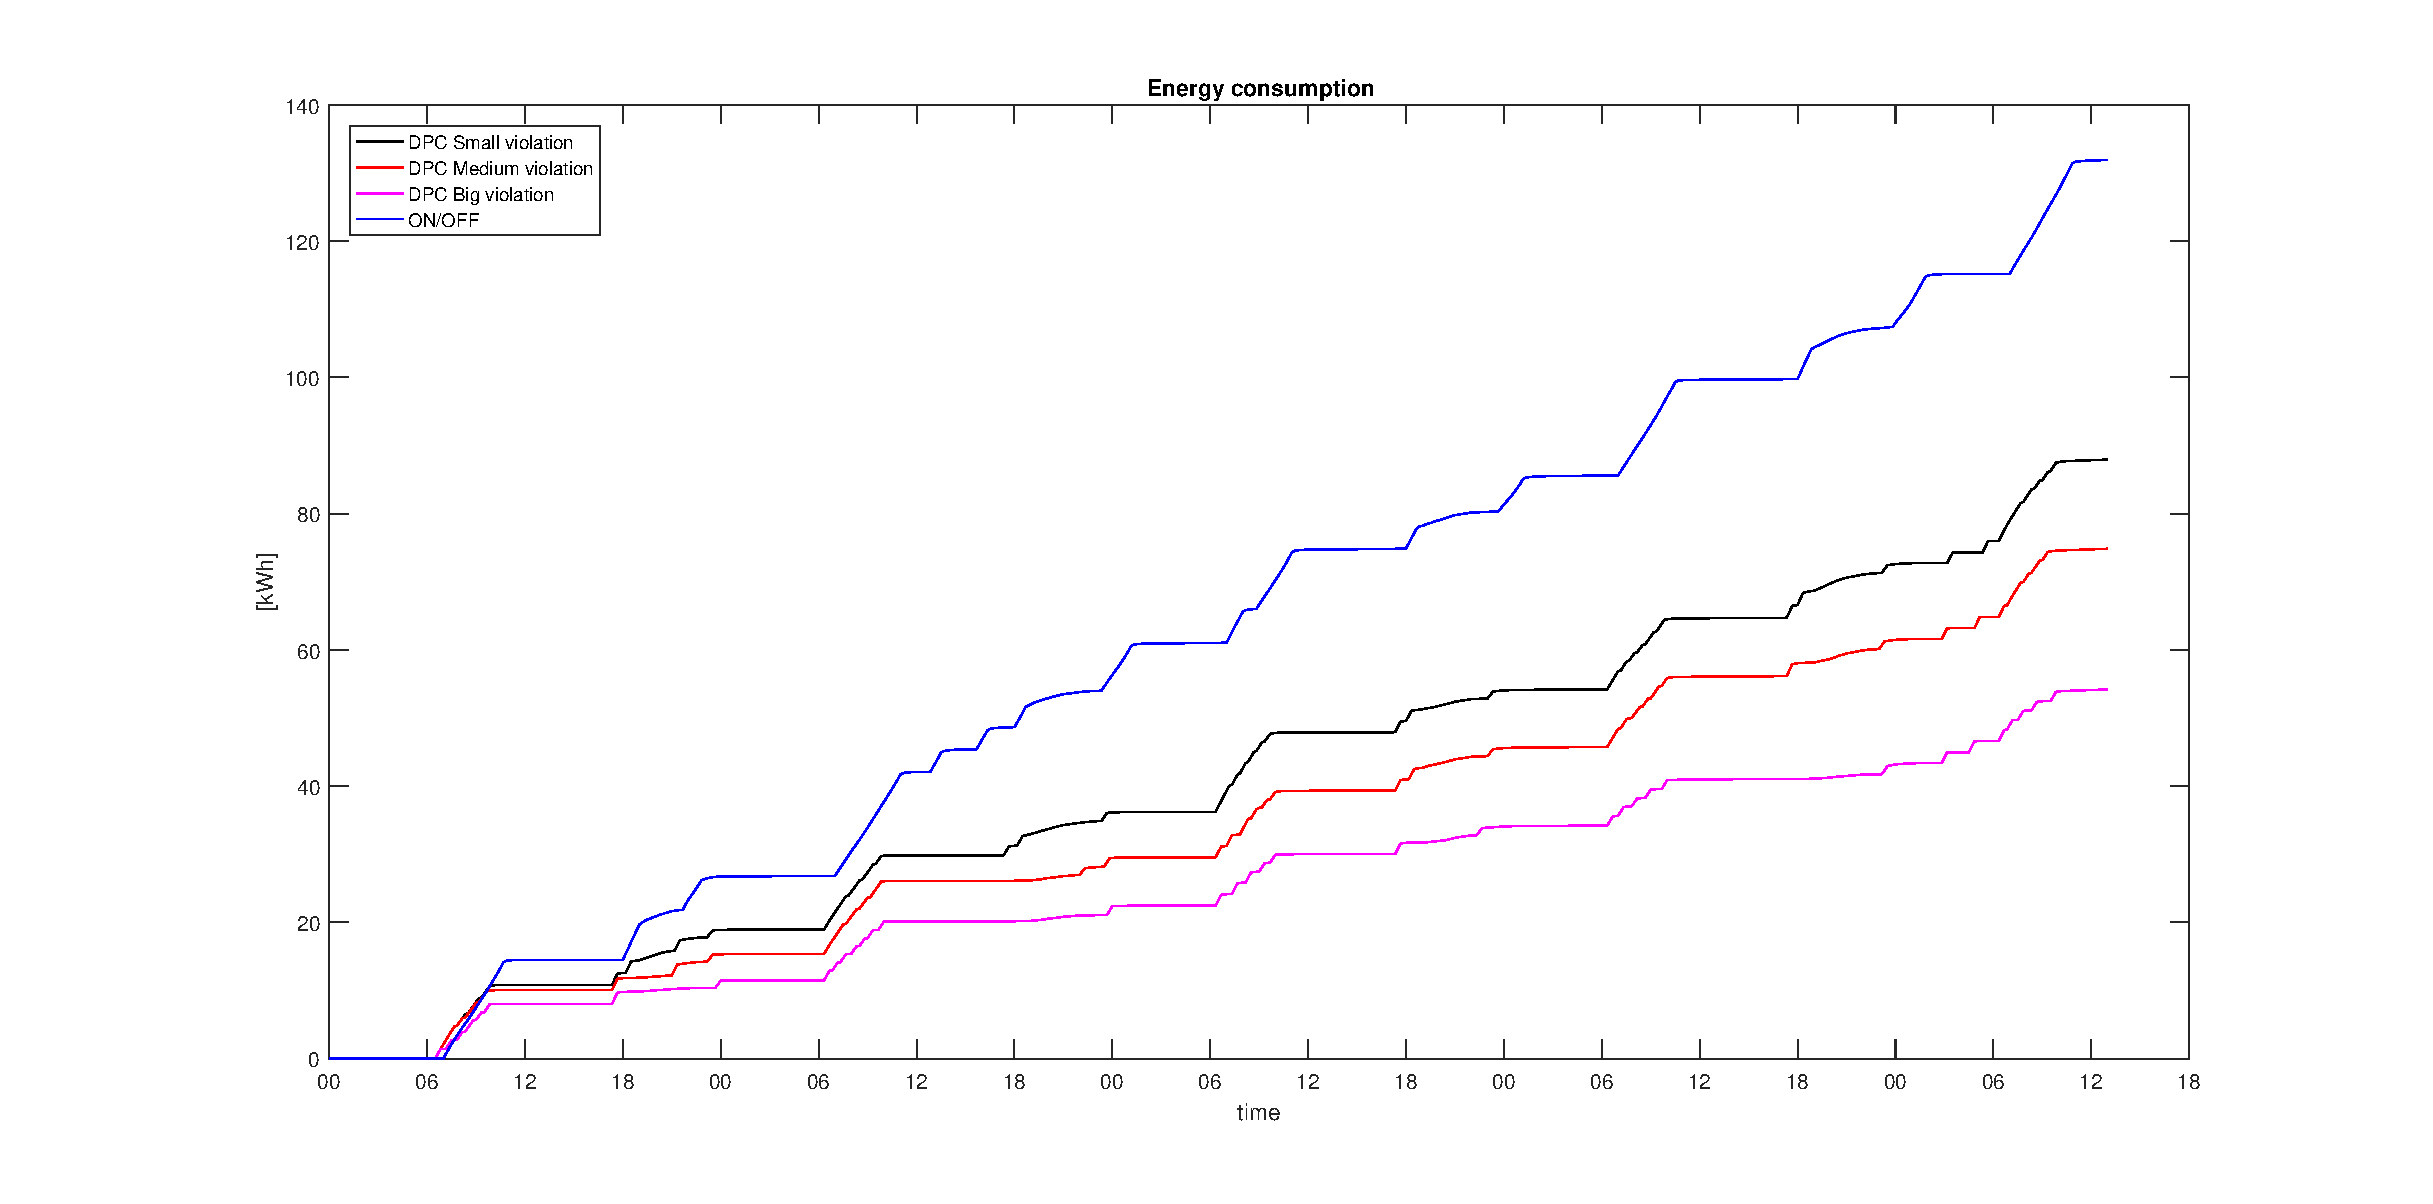
\includegraphics[width=26pc]{figures/Energy_all.eps}
	\end{center}
	\caption{Comparison of DPC and bang-bang control performance with different violations using random forest model.}
	\label{F:comparison_all_energy}
\end{figure}
An alternative comparison can be done considering the EnergyPlus model of the house for energy consumption described in Section \ref{SS:energyPlusmodel}. Results are shown in Figure \ref{F:comparison_all_energy_E+}.
\begin{figure}[h!]
	\begin{center}
		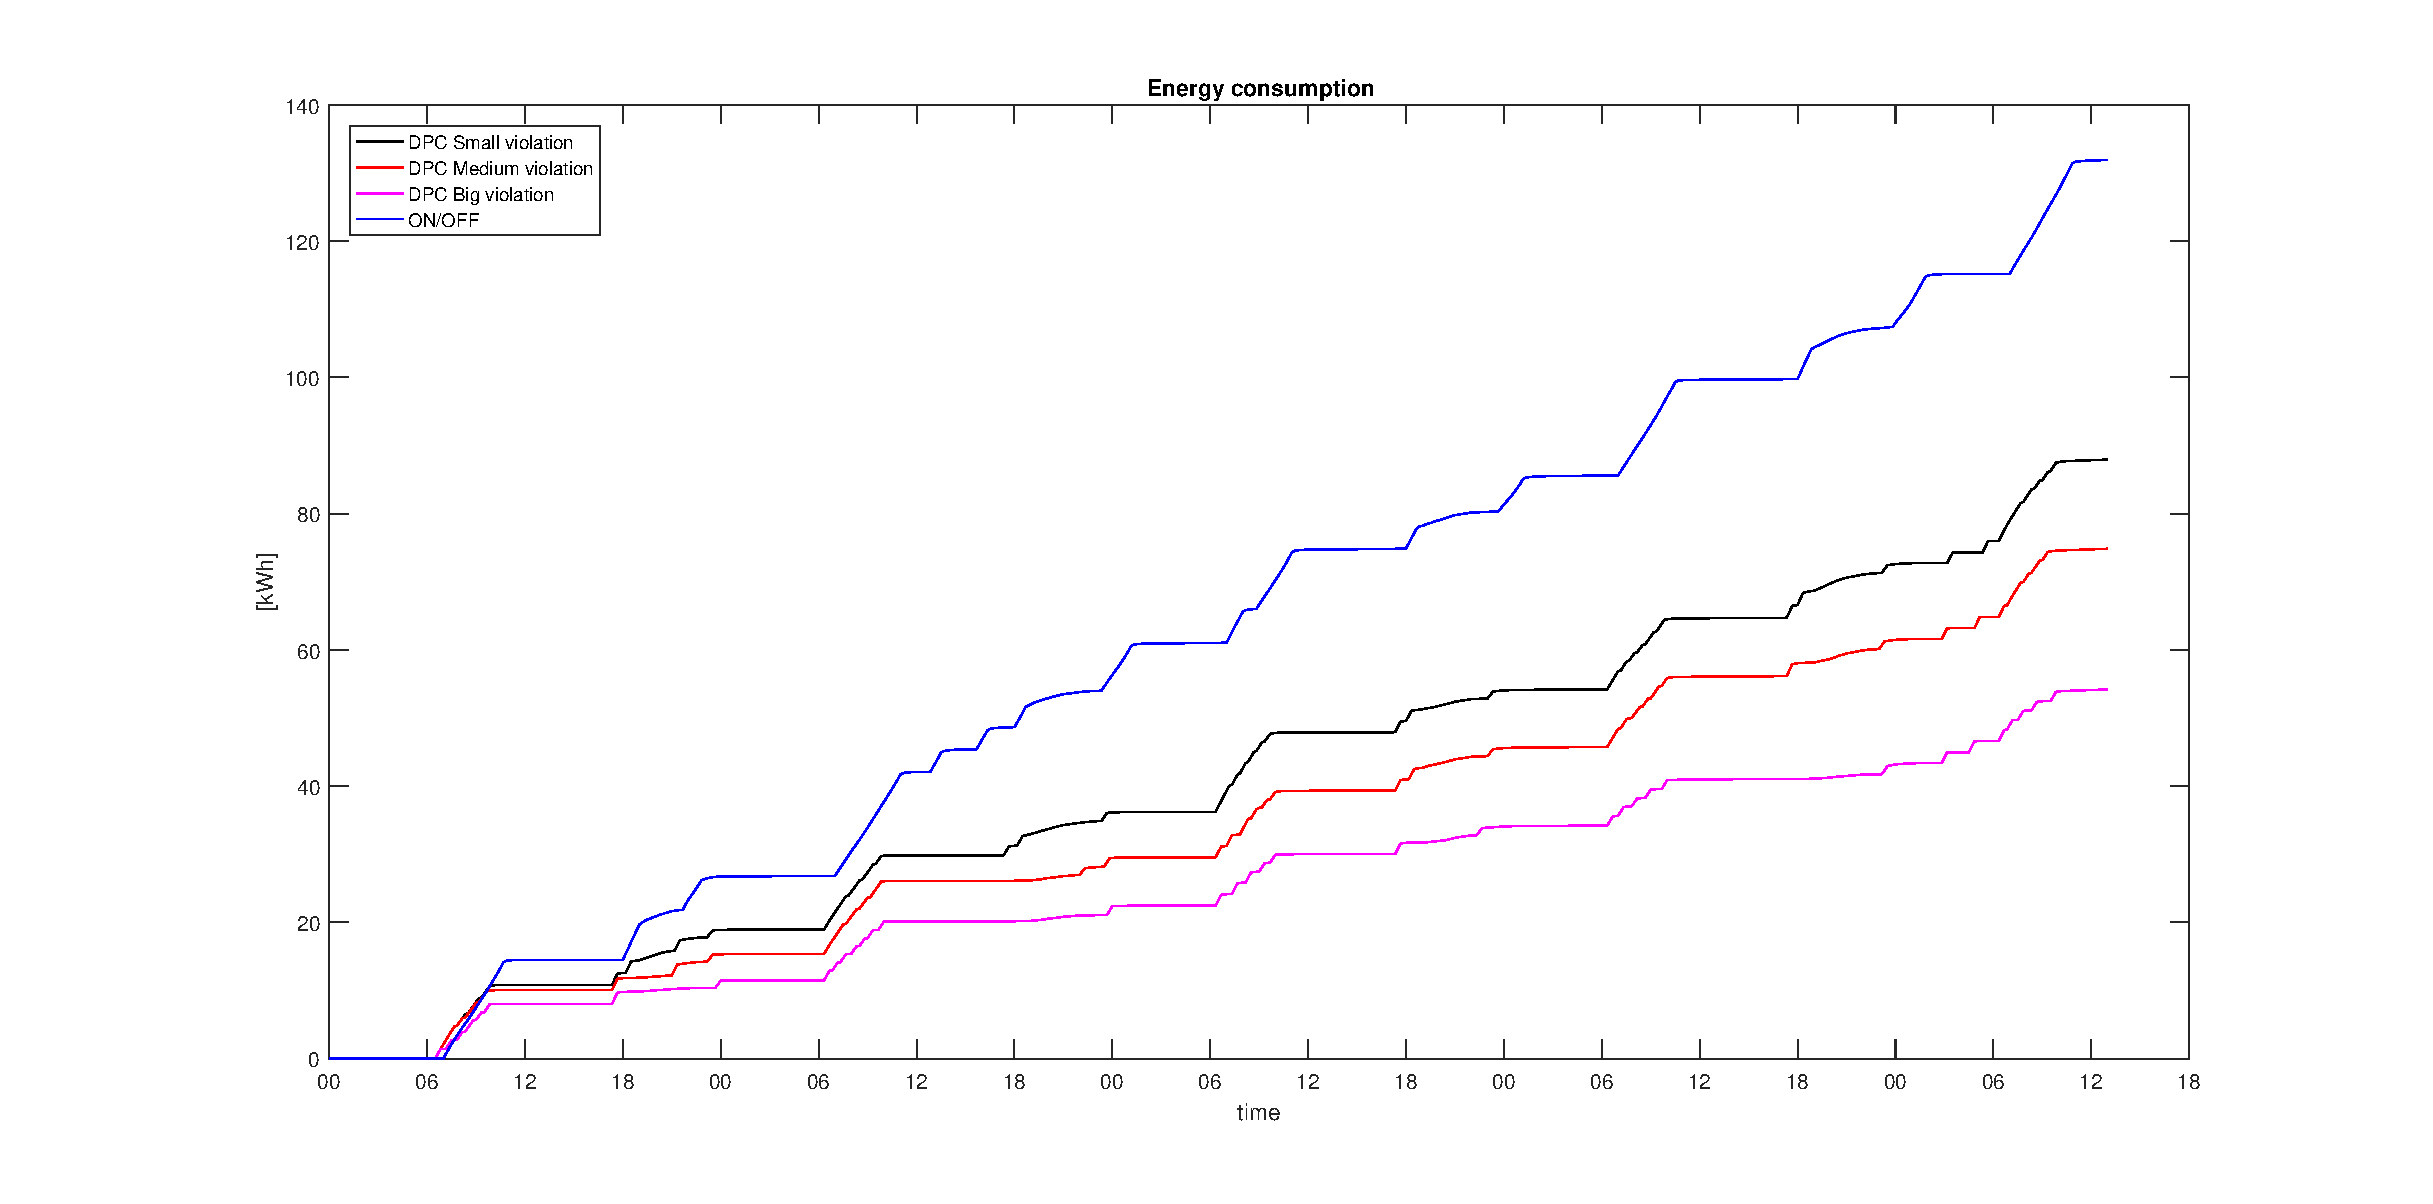
\includegraphics[width=26pc]{figures/Energy_all.eps}
	\end{center}
	\caption{SUBSTITUTE WITH TULLIO'S RESULTS Comparison of DPC and bang-bang control performance with different violations using EnergyPlus model.}
	\label{F:comparison_all_energy_E+}
\end{figure}
\textbf{TO BE ADAPTED WITH TULLIO'S RESULTS We can see that, over the same period of $4$ days and a half, using DPC we saved $TOT\, kWh$ allowing small violations, that correspond to a $TOT\%$ of energy saving, and $TOT\, kWh$ allowing large violations, that correspond to a $TOT\%$ of energy saving.}






